% =====================================================================
%  Capitolo 9 — Agency, comportamento dei giocatori e documenti di
%  visione: il paradosso della scelta, la Theory of Planned Behavior,
%  il compendium, la vision e la team vision, e un core elements rifatto
%  insieme (Game Design, primo anno)
%  Fonte: trascrizione della lezione GD9 (Game Design, primo anno),
%  lezione ibrida (in aula e da remoto). Non è una lezione di level
%  design: dopo la parentesi del capitolo 8 (Stefano Zocchi), torna il
%  docente delle lezioni di game design e documentazione dei capitoli
%  1--6, e la lezione si collega direttamente a quelle (framework di
%  Bura, atomo di Koster, production dictionary, core elements,
%  fine della pre-produzione).
%  Contenuti, nell'ordine della lezione: il problema di impostazione
%  pagina nel task di Pokémon; che cosa succede a un task non letto e
%  come si riconsegna; il limite dei cinque errori grammaticali e la
%  dislessia; la libertà non esiste, esiste l'agency (starter, build,
%  quattro mosse, stun lock e crowd control); il carretto dei dolci e i
%  cereali; gli skill tree (Path of Exile, Salt and Sanctuary); la
%  paura di scegliere e la fallacia di Monte Carlo; rimborsi e scelte
%  permanenti; il paradosso della scelta di Barry Schwartz; meno scelte
%  ma più profonde (Ori and the Blind Forest); la Theory of Planned
%  Behavior: attitudine, norme soggettive (sociali e meta: i colori di
%  Magic), perceived behavioral control (confidence e capability), le
%  barriere; la formula semplificata e i pesi; l'esempio di Valorant e
%  il survey su Reddit; il feedback; la situational awareness; la
%  pausa; il compendium (o design bible); i pilastri di God of War; la
%  vision; la team vision; le domande di fine pre-produzione; i template
%  come linee guida; l'esercizio in classe: i core elements di Frogger
%  scritti da uno studente e riformattati dal docente.
%  Integrazioni da "The Art of Game Design" (Jesse Schell), segnalate
%  come approfondimenti.
%
%  Pacchetti richiesti nel preambolo del libro (già presenti nel
%  main.tex): \usepackage{booktabs}, \usepackage{amsmath},
%  \usepackage{tikz} con
%    \usetikzlibrary{shapes.geometric,shapes.symbols,shapes.misc,
%      arrows.meta,positioning,calc,fit}
%  (le librerie vanno caricate nel preambolo, non nel capitolo).
%  Tutte le etichette di questo capitolo hanno il prefisso "gd9:"
%  (gd9:sec:..., gd9:fig:..., gd9:tab:...) e tutti gli stili TikZ il
%  prefisso "gd9", per non collidere con gli altri capitoli.
%
%  Nota sulla fonte: la trascrizione automatica è buona nella parte
%  teorica e molto rovinata nell'ultima ora. Le due pause sono state
%  trascritte come un'unica frase ripetuta in loop ("Grazie a tutti per
%  l'attenzione... Qual è la risposta che ci può essere?"), e un tratto
%  della spiegazione sulle barriere come "È una barriera meccanica"
%  ripetuto decine di volte: sono artefatti, omessi. L'esercizio finale
%  (uno studente al computer del docente, la classe che detta) è in gran
%  parte incomprensibile: si riporta solo ciò che è ricostruibile con
%  certezza, e si segnala in nota ciò che non lo è. Molti nomi propri
%  (di giochi, persone, strumenti) sono storpiati: dove il riferimento è
%  ricostruibile con certezza lo si riporta nella forma corretta; dove
%  non lo è, lo si segnala in nota invece di indovinare. Le figure sono
%  ricostruzioni schematiche di ciò che è mostrato a lezione, non le
%  slide originali.
% =====================================================================

\chapter[Agency, comportamento e visione]{Agency, comportamento e visione:
perché i giocatori scelgono, e la bussola del progetto}
\label{gd9:cap:agency-visione}

Dopo la parentesi del capitolo precedente, che era in realtà la prima lezione
del corso di level design (capitolo~\ref{gd8:cap:leveldesign}), si torna al
corso di game design vero e proprio, con il docente dei primi sei capitoli. Il
filo riprende esattamente da dove era stato lasciato: il production dictionary
(sezione~\ref{sec:production-dictionary}), i \emph{core elements}
(capitolo~\ref{cap:che-cos-e-un-gioco}), la fine della pre-produzione e la
\emph{game vision} (sezione~\ref{sec:fine-preproduzione}).

Il docente stesso annuncia che quella di oggi è, in realtà, \textbf{due
lezioni in una}: ``una lezione di documentazione, \emph{teaching}, e una
lezione di design e \emph{tools}''. ``Dovremmo riuscire a fare tutte e due,
realisticamente. Scopriremo a breve.'' Ci riesce, e la giornata si chiude
perfino con un esercizio dal vivo. La struttura della lezione, e quindi del
capitolo, è questa:
\begin{enumerate}
  \item le questioni pratiche in apertura: un problema di impostazione
        pagina nel task di Pokémon, che cosa succede a un task \textbf{non
        letto} e come lo si \textbf{riconsegna}, il limite dei cinque errori
        grammaticali (sezione~\ref{gd9:sec:apertura});
  \item la \textbf{libertà} che non esiste e l'\textbf{agency} che invece si
        progetta (sezione~\ref{gd9:sec:agency});
  \item il \textbf{paradosso della scelta}: perché troppe scelte rendono
        infelici, e che cosa se ne ricava come designer
        (sezioni~\ref{gd9:sec:troppe-scelte}
        e~\ref{gd9:sec:paradosso});
  \item la \textbf{Theory of Planned Behavior}: come i giocatori prendono
        le loro decisioni, con le sue sei componenti, le barriere e una
        formula per stimare un comportamento
        (sezioni~\ref{gd9:sec:tpb}--\ref{gd9:sec:valorant});
  \item il \textbf{feedback} che rinforza i comportamenti e la
        \textbf{situational awareness} da cui la teoria proviene
        (sezione~\ref{gd9:sec:feedback-sa});
  \item dopo la pausa, la documentazione: il \textbf{compendium} (o
        \emph{design bible}), i \textbf{pilastri} di \emph{God of War}, il
        documento di \textbf{vision}, la \textbf{team vision} e le domande
        che chiudono la pre-produzione
        (sezioni~\ref{gd9:sec:compendium}--\ref{gd9:sec:template});
  \item l'esercizio finale: i \textbf{core elements di Frogger} scritti dal
        vivo da uno studente e poi riformattati dal docente
        (sezioni~\ref{gd9:sec:esercizio} e~\ref{gd9:sec:riformattazione}).
\end{enumerate}

% ---------------------------------------------------------------------
\section{In apertura: impaginazione, riconsegne, errori}
\label{gd9:sec:apertura}

\subsection{Prima di cominciare}

La registrazione parte sul solito rito delle lezioni ibride: il computer è
nuovo, le postazioni sono nuove, la webcam ha ``questo filtro molto triste,
molto GTA 4'', e per un paio di minuti il docente non sente chi è collegato da
casa (gli studenti remoti, tra loro, si sentono benissimo). Risolto il
problema, la solita richiesta: ``attivate le webcam, qualora voi non foste nel
mezzo dell'apocalisse zombie''.

\subsection{Un problema di impostazione pagina}

Prima che la lezione cominci, uno studente segnala un problema sul secondo
task consegnato, quello su Pokémon, che il docente non ha letto proprio perché
``i parametri erano sballati''. Lo studente spiega di aver impostato i margini
da \emph{File} $\rightarrow$ \emph{Impostazione pagina}, inserendo i valori
richiesti; ma su quel documento il risultato è stato sbagliato, e non sapeva
come correggerlo.

Il docente condivide lo schermo e individua il colpevole: la
``\textbf{spazzatura} all'interno del documento'', cioè un \textbf{rientro}
residuo (un'indentazione rimasta impostata sul testo) che falsava
l'impaginazione. La prova del nove è semplice: in un \textbf{documento
nuovo}, con la stessa procedura, i margini risultano giusti. Il problema,
quindi, non era nella procedura, ma in ciò che il vecchio documento si
portava dietro.

\paragraph{Sperimentate, e chiedete.} Il commento del docente vale in
generale: ``provate, sperimentatevi, non fermatevi al primo risultato
possibile''. E se ci sono dubbi, \textbf{chiedere} resta sempre una
possibilità valida. Con una precisazione onesta: il docente non avrà sempre
la risposta, e a volte, pur avendola, non potrà darla (perché trovarla da
soli fa parte dell'esercizio).

\subsection{Che cosa succede a un task non letto}

La seconda domanda, che anche Francesco aveva posto in privato, è quella che
interessa a tutti: \textbf{che cosa succede se un task non viene letto?} Le
regole erano state date alla prima lezione
(sezione~\ref{sec:task-feedback}); il docente le riprende e le precisa.
\begin{itemize}
  \item Un task \textbf{non letto} è perduto nel conteggio finale dei task.
  \item Ma non è perduto \textbf{per sempre}: lo si può voler
        \textbf{recuperare}. Lo stesso vale per un task che non si è
        riusciti a consegnare entro la scadenza.
  \item Il docente \textbf{accetta le riconsegne}. Non saranno ideali come
        consegna finale, cioè non avranno lo stesso peso pieno di una
        consegna puntuale nel computo finale, ma vengono contate.
\end{itemize}

\paragraph{Quante volte?} Una studentessa chiede quante volte si possa
ricevere un ``non leggo'' e poi riconsegnare, perché nelle consegne ``mi
perdo veramente tante cose''. La risposta è un numero preciso: fino al
\textbf{20\% dei task totali}. Resta poi una garanzia aggiuntiva: per il
passaggio all'anno successivo, un task \emph{consegnato e lavorato} ma non
letto viene comunque considerato diversamente da un task \emph{mai
consegnato}. Il caso citato è proprio quello della studentessa con il
production dictionary: ``hai lavorato, però io non te l'ho letto'', e questo
viene tenuto in considerazione. E a maggior ragione se poi lo si rifà e lo si
riconsegna.

\subsection{Come si riconsegna}

La procedura, mostrata aprendo la cartella dei task revisionati e prendendo
``a caso'' come esempio il task di Alberto, è la seguente.
\begin{enumerate}
  \item \textbf{Non modificate il vecchio documento.} Non si risolvono i
        commenti, non si corregge la vecchia task: il documento commentato
        resta com'è.
  \item Se ne crea una \textbf{copia} o, ``ancora meglio'', si crea un
        \textbf{documento da zero}.
  \item Lo si riempie includendo \textbf{tutto ciò che il docente ha
        commentato} (o non ha commentato) nel proprio task precedente,
        \textbf{più tutto ciò che ha commentato nei task dei colleghi}.
  \item Lo si inserisce nella \textbf{cartella di riferimento} del task
        (gli Arcade nella cartella degli Arcade, il production dictionary
        nella sua), o creando una sottocartella con \emph{cognome e nome},
        come aveva fatto Valerio con più documenti, o comunque con un
        \textbf{nome comprensibile} e in modo ordinato.
  \item Si \textbf{scrive al docente}, perché deve sapere che c'è una
        riconsegna. Poi si attendono di nuovo i commenti, che probabilmente
        non saranno rapidi come quelli di un task normale.
\end{enumerate}

\paragraph{Il task si riconsegna con ciò che si sa \emph{oggi}.} È il punto
più importante, e il docente lo sottolinea: chi riconsegna, per esempio, il
task sui core elements, non viene letto ``come se fosse fermo a quel punto
lì''. La riconsegna deve contenere \textbf{tutte le nozioni apprese anche
dopo}, cioè tutto ciò che si è accumulato fino al momento della nuova
consegna: i commenti propri, i commenti ai colleghi, ``tutte le altre cose
che ci siamo detti nel mentre''. Ed è questo che viene valutato.

\paragraph{Non riconsegnate il giorno dopo.} Da qui un invito esplicito: se
un task non viene letto, \textbf{non va riconsegnato il giorno dopo},
correggendo solo le cose commentate. Bisogna prendersi del tempo per capire,
ma anche per \textbf{leggere i task degli altri} e integrare ciò che si è
imparato, ``da lì a una settimana, due settimane, un mese''. Il docente
assume che nel task riconsegnato ci sia gran parte delle conoscenze apprese
fra la lettura e la riconsegna.

\subsection{Il limite dei cinque errori e la dislessia}

L'ultimo annuncio riguarda chi ha problemi di \textbf{dislessia} o difficoltà
associate. Ora che la classe ha visto ``con mano'' che cosa significa contare
gli errori nei task (il registro delle revisioni è nel
capitolo~\ref{rv:cap:errori-task}), il docente invita chiunque si trovi in
questa situazione (ne aveva già parlato con una studentessa e con Mattia) a
\textbf{scrivergli in privato}: il \textbf{limite dei cinque errori
grammaticali} (sezione~\ref{sec:regole-formali}) può essere sollevato. Con
due precisazioni.
\begin{itemize}
  \item Il motivo del limite è il ``mondo brutale là fuori''. Nei documenti
        operativi dei task non dovrebbe succedere (``almeno a me non è
        capitato; spero non succeda mai''), ma ci sono casi in cui la persona
        di riferimento si aggrappa a qualsiasi cosa per non leggere. Cinque
        errori grammaticali sono certamente rilevanti in un
        \textbf{curriculum} o in un \textbf{portfolio}: ``sappiatelo''.
  \item Chi ritiene che sollevare il limite gli faccia bene, viene
        accontentato; ma è una possibilità per chi ne ha bisogno, ``non è
        che adesso avanzate tutti questa possibilità''.
\end{itemize}

Il docente annuncia infine che nell'ultima ora si farà ``questa cosa di cui
magari qualcuno si è dimenticato; tuttavia io non dimentico, come gli
elefanti'': un volontario prenderà il posto del docente al computer e, ``con
il potere della forza e dell'amicizia'', creerà insieme alla classe un nuovo
documento di \textbf{core elements}, applicando tutto ciò che si è imparato
finora sulla formattazione (era l'impegno preso alla fine del
capitolo~\ref{cap:brainstorming-flowchart}, sezione~\ref{sec:chiusura-gd6}).
È l'esercizio delle sezioni~\ref{gd9:sec:esercizio}
e~\ref{gd9:sec:riformattazione}.

% ---------------------------------------------------------------------
\section{La libertà non esiste: esiste l'agency}
\label{gd9:sec:agency}

\subsection{Un concetto che ritorna da Bura}

Il primo argomento di design è la \textbf{libertà}. Non è un concetto nuovo:
compariva già nel framework di Stéphane Bura, nella colonna \emph{Freedom}
(sezione~\ref{sec:bura}, tabella~\ref{tab:bura}). Il docente ricorda di aver
detto, presentandolo, che quel framework è complesso e che alcuni dei suoi
aspetti sarebbero stati ``rivisti in altre cose, nel corso del corso'' (``e
scusate il gioco di parole''). La libertà è uno di questi.

\subsection{Ciò che le persone cercano davvero}

``Ogni giocatore, chiunque, vuole libertà.'' Il docente scherza sul fatto che
la battuta sulla libertà e sull'America ``ormai si spreca'' e, rimandando a
una GIF mostrata prima, dichiara subito che l'affermazione è \textbf{falsa}.
E non vale solo per i giocatori: vale per qualsiasi persona.

Ciò che le persone cercano non è la libertà in sé, ``concetto molto
esagerato, molto ampio e anche molto rattristante'' (si capirà perché nella
sezione~\ref{gd9:sec:paradosso}). Ciò che le persone cercano è
l'\textbf{agency}:
\begin{quote}
  la capacità, la condizione, lo stato di \textbf{esercitare potere entro
  alcuni limiti}.
\end{quote}
I limiti sono parte della definizione. È anche il motivo per cui la
definizione di gioco del docente ragiona sempre \textbf{entro i limiti del
sistema}, entro le regole del sistema (sezione~\ref{sec:framework-direttore}).
Nel caso dei videogiochi, e dei giochi in generale, quei limiti li stabilisce
il \textbf{designer}.

\paragraph{Una regola di vocabolario.} Da qui in avanti, nel corso,
``libertà'' come termine \textbf{non esiste}. ``Non è così grave come
\emph{divertente}'' (la parola proibita, sezione~\ref{rv:t1:sec:linguaggio}),
``però avete capito'': il termine corretto, ciò che si va a cercare, è
\textbf{agency}.

\subsection{Esempi di agency}

\begin{description}
  \item[La scelta dello starter] in Pokémon è ``l'esempio ideale, proprio
        l'esempio perfetto''. Ed è il motivo per cui gli starter sono
        \textbf{tre}.
  \item[La scelta della build iniziale] in \emph{Dark Souls}, all'inizio del
        gioco, dove le scelte sono estremamente limitate.
  \item[Le quattro mosse] ancora in Pokémon, ``che avete analizzato di
        recente'': in battaglia si possono scegliere \textbf{quattro} mosse.
        Non 27, non 10: quattro.
  \item[I sistemi di combattimento] molti si basano su pochi elementi:
        schivata; attacco (leggero, pesante, la combo da tre colpi, l'attacco
        caricato); parata o \emph{parry}. Bene o male: offesa, schivata,
        difesa.
\end{description}

\subsection{E il contrario: togliere agency}

Vale anche il contrario: tutto ciò che limita la possibilità di agire e di
scegliere del giocatore \textbf{toglie agency}.
\begin{itemize}
  \item Lo \textbf{stun lock}:\footnote{Nella trascrizione ``di Stan
        Lock''; dal contesto (il giocatore bloccato in combattimento) si
        tratta quasi certamente dello \emph{stun lock}, la condizione in cui
        un personaggio viene stordito ripetutamente senza poter reagire.}
        sto combattendo e vengo trasformato in una pecorella che non può fare
        nulla, se non muoversi e saltellare in giro.
  \item In \emph{League of Legends}, subire \textbf{CC} (\emph{crowd
        control}): rimanere fermi senza poter usare nessuna abilità né fare
        nessun movimento, ``sono lì a prendere pizze''.
\end{itemize}
Sono esempi di \textbf{agency assente} o \textbf{limitata}, tolta al
giocatore. Ciò che interessa al designer, però, è il discorso positivo:
come si dà agency.

\paragraph{Approfondimento: la sensazione di libertà.} Jesse Schell dedica
alla libertà una lente intera, la \emph{Lens of Freedom} (lente n.~79), e
arriva a una conclusione molto vicina a quella del docente. Non bisogna
sempre dare al giocatore \emph{vera} libertà: basta dargli la
\textbf{sensazione} di libertà. Se un designer abile riesce a far sentire
libero un giocatore che in realtà ha pochissime scelte, si ottiene il meglio
dei due mondi: il giocatore ha l'esperienza dell'agency, e il designer
controlla l'esperienza in modo economico. Le domande della lente: quando i
giocatori hanno libertà d'azione, e si sentono liberi in quei momenti? Quando
sono vincolati, e si sentono vincolati? Dove li si potrebbe far sentire più
liberi? E dove, al contrario, sono \textbf{sopraffatti da troppa
libertà}?\footnote{Jesse Schell, \emph{The Art of Game Design: A Book of
Lenses}, terza edizione, cap.~18 (\emph{Indirect Control}).}

% ---------------------------------------------------------------------
\section{Troppe scelte: il carretto, i cereali, gli skill tree}
\label{gd9:sec:troppe-scelte}

\subsection{Il carretto dei dolci}

Per rendere il discorso concreto, il docente propone un esperimento
mentale (``e peggio per voi che siete a casa''): qui fuori c'è un carrettino
con \textbf{cioccolato gratis}, \textbf{gelato gratis} e \textbf{torta di
mele gratis}. (``Non è vero, per chi se lo stesse chiedendo: non c'è il
carrettino, purtroppo.'') Uno a testa. Chi vuole il cioccolato? Chi il
gelato? Chi la torta?

Le mani si alzano: il gelato parte basso e poi sale, ``due persone, tre
persone, quattro persone, credibile''. Federica non vuole niente: non le
piacciono molto i dolci. ``Si può non scegliere?'' Sì, e il docente nota che
\textbf{non scegliere è una quarta possibilità} che le concede. (``Uno a
testa, quindi la torta di Federica me la prendo io, e mangerò due torte di
mele.'') La scelta è stata facile: ognuno è ``caduto sulla sua preferenza'',
o non preferenza.

\subsection{I cereali}

Seconda domanda: ``scegliete una marca di cereali a vostro piacimento''. Il
docente mostra un'immagine con molte scatole di cereali e mette fretta:
``Francesco, veloce, fai una scelta''. Francesco sceglie dei \emph{Pops};
Antonino un altro tipo.\footnote{Nella trascrizione la scelta di Antonino
compare come ``Titanino'', non riconoscibile.} ``E già vi ho dato un'altra
limitazione, che è il \textbf{tempo}.''

Poi la provocazione: ``Francesco, sei sicuro della tua scelta? Anche se qui
c'erano i cereali di \textbf{Gizmo}, dei \emph{Gremlins}? E quelli di
\textbf{Mr.~T}? Non ti sarebbero piaciuti?'' Nessuno aveva visto i cereali
dei Gremlins, ``nascosti'' tra gli altri (il docente confessa un debole per
Gizmo). Il punto è questo: anche questa scelta è più o meno limitata, ma
\textbf{molto maggiore} rispetto alle tre del carretto. E con più opzioni
aumenta il rischio di \textbf{non vedere} l'opzione che si sarebbe preferita,
e di dubitare della propria scelta dopo averla fatta.

\subsection{Gli skill tree}

Il concetto ``si può espandere molto''. È la differenza tra uno skill tree
contenuto e uno sterminato. Il docente mostra prima uno skill tree
``abbastanza contenuto'' (il riferimento è a \emph{Star Wars Jedi: Fallen
Order})\footnote{Nella trascrizione ``Following Order'': quasi certamente
\emph{Star Wars Jedi: Fallen Order} (2019), che ha uno skill tree
relativamente piccolo. Il passaggio è confuso e in parte contraddittorio
(``No, no, non Star Wars''), quindi l'attribuzione resta un'ipotesi.} e poi
quello di \textbf{\emph{Path of Exile}}, ``il Diablo-like'', famoso per il suo
albero passivo gigantesco; poi un terzo, ``intermedio'', sicuramente più
piccolo.\footnote{Il gioco dello skill tree intermedio compare nella
trascrizione come ``Paolo Zolaico'', non riconoscibile.} In quasi tutti ci
sono delle limitazioni: la classe scelta all'inizio indirizza già verso un
ramo o un altro. Ma diventa chiaramente complesso \textbf{leggere} un albero
del genere, o anche solo muoversi nella decisione.

\paragraph{Il rischio di pentirsi.} Il rischio è di investire punti e
risorse in un ramo e \textbf{pentirsene} dopo: perché la scelta ottimale era
altrove, perché il proprio stile di gioco è cambiato, o perché nel frattempo
si sono ottenute più informazioni sul gioco, sulle meccaniche, sui sistemi.
(Uno studente ricorda che in Path of Exile esiste un meccanismo per tornare
indietro; il docente non lo ricorda con certezza, e comunque il problema è a
monte.)

\paragraph{Il problema è in partenza.} Al netto di qualsiasi meccanica di
rimborso, il problema è l'impatto: ``immaginate che io entro in Path of Exile,
apro lo skill tree e mi trovo davanti questa roba''. Lo stesso valeva per
\textbf{\emph{Salt and Sanctuary}},\footnote{Nella trascrizione ``Salt and
Sentry''.} giocato dal docente in co-op locale: lui voleva fare il mago,
l'amico il paladino, e all'inizio era complesso capire quale ramo
ottimizzare, per di più ragionando su due giocatori. Nel peggiore dei casi
si rimane \textbf{impietriti} davanti alle possibilità: bloccati.

\subsection{Il cervello non è fatto per i grandi numeri}

Il nostro cervello non è ottimizzato per ragionare su grandi numeri, ed è lo
stesso motivo per cui non sappiamo leggere correttamente la probabilità
statistica. Il docente cita un bias che si vedrà al secondo anno, che chiama
``effetto Monte Carlo'':\footnote{Il nome corretto è \textbf{fallacia di
Monte Carlo}, nota anche come \emph{fallacia del giocatore} (\emph{gambler's
fallacy}): la convinzione che eventi indipendenti passati influenzino la
probabilità di quelli futuri. Prende il nome da un episodio del 1913 al
casinò di Monte Carlo, in cui il nero uscì alla roulette ventisei volte di
fila.} vado al casinò, alla roulette; oggi esce il 4 rosso, domani esce il 4
rosso, dopodomani esce il 4 rosso. Il quarto giorno ``probabilmente non
uscirà più'', pensiamo: la probabilità che esca di nuovo ci sembra più bassa.
``Ma non è che funzioni proprio così, la statistica'': ogni giro è
indipendente, e la probabilità resta la stessa. È un \textbf{bias
cognitivo}, e mostra che il cervello non è così pronto a ragionare
logicamente.

\subsection{La paura di scegliere, e il rimorso}

Mettere un giocatore davanti a un'enorme quantità di scelte, quindi, non solo
può tenerlo \textbf{fermo}: genera
\begin{itemize}
  \item la \textbf{paura di scegliere}, cioè di scegliere in maniera
        sbagliata (più o meno sentita a seconda dell'individuo, ma esiste);
  \item il \textbf{rimorso} di aver scelto sbagliato, un domani.
\end{itemize}

\subsection{Rimborsi e scelte permanenti}

Una meccanica che può rimediare, più o meno, al problema è quella che
suggeriva Francesco: \textbf{rimborsare}, permettere di tornare sui propri
passi (il \emph{respec}). Ma questo apre un altro problema, di cui si parlerà
in una lezione successiva: \textbf{se una scelta non è permanente, il
giocatore la percepisce come non così importante}, non così pesante. Le scelte
narrative memorabili che ciascuno ricorda, in qualsiasi gioco, generalmente
erano \textbf{irreversibili}: scegliere tra far vivere il personaggio X o il
personaggio Y, o scegliere una classe che non si può più cambiare e che
cambia tutto il gameplay dall'inizio alla fine.

Ci sono quindi una serie di rischi nel dare ``così tanta libertà'' al
giocatore; anzi, di libertà non si parla: si ragiona sempre dentro alcuni
limiti, che sono dati dal designer.

% ---------------------------------------------------------------------
\section{Il paradosso della scelta}
\label{gd9:sec:paradosso}

\subsection{Più scelte, più infelicità}

Questo fenomeno ha un nome: il \textbf{paradosso della scelta}. Più scelte si
danno a una persona (a un giocatore, ma in generale a chiunque), più c'è il
rischio che quella persona si senta, ``sto esagerando, sto astraendo'',
\textbf{infelice}. È un concetto studiato molte volte, diventato
particolarmente visibile nel panorama americano.\footnote{Nella trascrizione
``studiato \ldots{} dai comunisti americani'': quasi certamente una
storpiatura (forse ``economisti'' o ``psicologi''); non è ricostruibile con
certezza.}

Il docente legge alcune citazioni dal libro \textbf{\emph{The Paradox of
Choice}} (\emph{Il paradosso della scelta}) dello psicologo americano
\textbf{Barry Schwartz}:\footnote{Barry Schwartz, \emph{The Paradox of
Choice: Why More Is Less}, 2004. Il nome dell'autore non compare nella
trascrizione, ma il titolo e le citazioni corrispondono.}
\begin{quote}
  Autonomia e libertà di scelta sono critiche per il nostro benessere, e la
  scelta è critica per la libertà e l'autonomia. Eppure, sebbene gli
  americani moderni abbiano più scelta di qualsiasi altro gruppo di persone
  prima di loro, e quindi, presumibilmente, più libertà e autonomia, non
  sembriamo trarne beneficio psicologico.
\end{quote}
Sulla prima parte ``siamo tutti d'accordo'': gli esseri umani tendono verso
la libertà, e non a caso il sistema giudiziario punisce le persone con il
carcere, cioè \textbf{togliendo libertà}. Il problema è la seconda parte:
una \textbf{grande} libertà di scelta può provocare infelicità, perché ci si
sente \textbf{meno soddisfatti} del risultato di una scelta fatta tra molte
opzioni di quanto lo si sarebbe stati con meno opzioni. Con tre opzioni,
A, B e C, è più facile ottimizzare il risultato, e c'è meno possibilità che
esistesse un percorso migliore, anche solo leggermente migliore, che non si
è preso.

\paragraph{Le basse aspettative.} Un'altra citazione dal libro:
\begin{quote}
  Il segreto della felicità sono le basse aspettative.
\end{quote}

\paragraph{Gli atleti olimpici.} E un altro risultato citato: tra gli atleti
sul podio olimpico, i più felici sono l'\textbf{oro} e il
\textbf{bronzo}.\footnote{Il riferimento è allo studio di Victoria Medvec,
Scott Madey e Thomas Gilovich (1995) sulle espressioni dei medagliati alle
Olimpiadi di Barcellona del 1992, che trovò i medagliati di bronzo
mediamente più soddisfatti di quelli d'argento.} Il bronzo è ``saltato'' dal
quarto posto, che generalmente nessuno ricorda, al terzo, ed è stato
premiato; il secondo, si suol dire, è ``il primo degli ultimi''. Tutto
dipende dal termine di paragone, e quindi dalle aspettative.

Il risultato di tutto questo è sempre lo stesso: \textbf{bassa felicità}, o
comunque \textbf{insoddisfazione} dell'utente.

\subsection{Che cosa ce ne facciamo come designer}

``Non parleremo sempre di videogiochi'', ma la domanda è: come aiuta, questo
concetto? Il paradosso della scelta è utile da tenere in considerazione ogni
volta che si parla di agency e di \textbf{possibilità limitate date al
giocatore}. Se lo si tiene presente, si può aumentare l'agency del giocatore
e, soprattutto, la \textbf{qualità} dell'agency che gli si dà: \textbf{meno
scelte, ma più profonde}.

E come si raggiunge una scelta più profonda? Con un design migliore:
impiegando le risorse su \textbf{tre sistemi invece che su cento}, si può
iterare molto di più, ``perché sono tre e non cento''. I vantaggi, che il
docente elenca da una slide, stanno su due fronti (tabella~\ref{gd9:tab:less-is-more}).

\begin{table}[htbp]
  \centering
  \caption{\emph{Less is more}: i vantaggi di dare meno scelte, ma più
  profonde.}
  \label{gd9:tab:less-is-more}
  \small
  \begin{tabular}{@{}p{0.45\textwidth}p{0.45\textwidth}@{}}
    \toprule
    \textbf{Per il giocatore} & \textbf{Per il progetto} \\
    \midrule
    Aumenta la \textbf{soddisfazione percepita}: meno blocco, meno paura di
    agire davanti a una quantità esagerata di scelte. &
    \textbf{Riduzione a monte} della grandezza del progetto: meno cose di
    cui preoccuparsi in produzione, prima e dopo. \\
    \addlinespace
    Si riduce la \textbf{curva d'apprendimento}: poche scelte all'inizio,
    di più quando il giocatore ha sviluppato \emph{mastery}. &
    Più \textbf{risorse} di produzione dedicate a \textbf{meno cose}: costo
    ridotto, più iterazione. \\
    \addlinespace
    Decisioni \textbf{meaningful}: scelte meno numerose, quindi più
    dettagliate e percepite come più importanti. &
    \textbf{Potenzia la creatività}: ragionare con pochi sistemi porta a un
    risultato migliore dal punto di vista del design. \\
    \addlinespace
    \textbf{Scelte migliori}: scegliendo in una gamma più ridotta, il
    giocatore è più soddisfatto. &
    Design più \textbf{bilanciato}: si bilanciano 3, 5, 10 elementi invece
    di 10\,000. \\
    \bottomrule
  \end{tabular}
\end{table}

\paragraph{Ridurre la curva d'apprendimento non vuol dire dare sempre poco.}
Il docente precisa: non significa che si debba sempre dare un numero limitato
di scelte. Lo si può \textbf{incrementare nel tempo}: poche scelte all'inizio,
di più quando il giocatore ha sviluppato \emph{mastery} sui sistemi.
L'esempio, ``una chiacchiera da bar, che bisognerebbe analizzare meglio'', è
\textbf{\emph{Ori and the Blind Forest}}:\footnote{Nella trascrizione
``Orient e Blind Forest''.} all'inizio dà pochi sistemi di locomozione e poi
spinge la curva, che il docente corregge a voce da ``molto ripida'' a
``\textbf{molto morbida}''. La progressione di quel gioco, soprattutto sul
fronte della mastery, è per il docente un punto di riferimento ideale per i
platformer. Tra l'altro ha una meccanica che si basa sul colpire i
\textbf{proiettili dei nemici per saltare più in alto},\footnote{Il docente
la descrive come un \emph{parry}; nel gioco l'abilità si chiama
\emph{Bash}, e permette di aggrapparsi per un istante a un nemico o a un
proiettile e di lanciarsi nella direzione opposta, rilanciando il proiettile.}
cosa che in molti altri giochi ``sarebbe stata disastrosa''.

\paragraph{Decisioni meaningful.} Dare meno scelte permette al giocatore di
percepire \textbf{in maniera più importante} le scelte che adotta, perché
sono meno e quindi possono avere più dettaglio, più iterazione. Non è
l'unico ingrediente per rendere una decisione meaningful, ``non è l'unica
discriminante'': è un discorso che verrà ripreso più avanti nel corso.

\paragraph{Tre è un ottimo punto di partenza.} Dal lato del progetto, il
grande vantaggio è il costo ridotto, le risorse risparmiate; ma, di contro,
il limite \textbf{potenzia la creatività}. Ragionare in maniera limitata, non
dover produrre mille sistemi ma tre, quattro, cinque, permette di raggiungere
un risultato migliore e sicuramente più \textbf{bilanciato}. ``Tre è un
ottimo punto di partenza: non a caso gli starter sono tre, in ogni gioco.''
(Una mano si alza; era solo ``una grattata''.)

\paragraph{Approfondimento: quante scelte dare.} Schell, nel capitolo sul
bilanciamento, cita un'osservazione di Michael Mateas: il numero di scelte che
un giocatore cerca dipende dal numero di cose che \textbf{desidera} fare.
\begin{itemize}
  \item se le scelte sono \textbf{più} dei desideri, il giocatore è
        \textbf{sopraffatto};
  \item se le scelte sono \textbf{meno} dei desideri, il giocatore è
        \textbf{frustrato};
  \item se scelte e desideri coincidono, il giocatore prova una sensazione
        di \textbf{libertà} e di appagamento.
\end{itemize}
Scegliere tra la strada di sinistra e quella di destra è interessante;
scegliere tra trenta stradine laterali è opprimente. Altre volte, invece, il
giocatore desidera moltissime opzioni (l'esempio di Schell è il negozio di
vestiti dei \emph{Sims}). Schell aggiunge due trappole speculari: offrire
scelte \textbf{prive di significato} (cinquanta auto che si guidano tutte
allo stesso modo equivalgono a nessuna scelta) e offrire scelte che
\textbf{nessuno vorrebbe} (dieci armi di cui una è chiaramente migliore: una
\emph{strategia dominante}). Ne nasce la \emph{Lens of Meaningful Choices}
(lente n.~39): quali scelte chiedo al giocatore? Sono significative, e
perché? Gli sto dando il numero giusto di scelte, e ne servirebbero di più
per farlo sentire potente, o di meno per rendere il gioco più
chiaro?\footnote{Schell, \emph{The Art of Game Design}, cap.~13.}

\paragraph{Approfondimento: il vincolo come controllo indiretto.} Nello
stesso spirito, Schell elenca il \textbf{vincolo} (\emph{constraint}) come
primo metodo di controllo indiretto. ``Scegli un colore'' e ``scegli un
colore: rosso, blu o verde'' danno entrambi libertà di scelta, ma il secondo
riduce le risposte possibili da milioni a tre, e chi avrebbe comunque scelto
uno dei tre non nota nemmeno la differenza. Il suo aneddoto ricorda il
carretto dei dolci: lavorando in un negozio di caramelle con sessanta gusti,
recitarli tutti spaventava i clienti, e chiedere ``dimmi tu il gusto che
vuoi'' li bloccava; funzionava invece dire ``abbiamo quasi tutti i gusti, ma
i più richiesti sono questi sei''. I clienti si sentivano liberi, ma avevano
davanti poche opzioni chiare, e sceglievano.\footnote{Schell, \emph{The Art
of Game Design}, cap.~18.}

% ---------------------------------------------------------------------
\section{Come decidono i giocatori: la Theory of Planned Behavior}
\label{gd9:sec:tpb}

\subsection{Un framework per leggere i comportamenti}

Fin qui si è parlato di \emph{less is more} e di agency. Ora si aggiunge un
pezzo: \textbf{come i giocatori prendono le loro decisioni}. Il framework
``arriva direttamente dal secondo anno'' ed è un inserimento recente nel
programma: è ``un'altra delle cose che finirà nella vostra cintura''. Non lo
si deve usare per forza, ma comincia già a dare informazioni su come i
giocatori scelgono.

Ci si può fare design, come con quasi tutti i framework. Ma l'opinione del
docente è che il suo vero uso sia l'\textbf{analisi}, e in particolare
l'\textbf{analisi da playtest}: leggere come i giocatori hanno fatto, o
``ancora meglio, \textbf{non} hanno fatto'', alcune cose che il designer
aveva previsto nel gioco, e perché. Serve soprattutto a \textbf{spiegare
perché alcuni comportamenti vengono adottati e altri no}: brilla nella
\emph{data analysis}.

Il framework è la \textbf{Theory of Planned Behavior}
(TPB),\footnote{Nella trascrizione il nome è storpiato in molti modi
(``Tier of Planned Behavior'', ``Team of Planned Behavior'', ``Tierra of
Planned Behavior''). La teoria del comportamento pianificato è stata
formulata dallo psicologo sociale Icek Ajzen (1985--1991), come estensione
della teoria dell'azione ragionata. La suddivisione di ciascun fattore in due
sotto-componenti, le barriere e la formula numerica delle
sezioni~\ref{gd9:sec:tpb-barriere} e~\ref{gd9:sec:formula} sono una versione
semplificata e adattata ai giochi presentata a lezione, non la formulazione
originale di Ajzen.} che il docente presenta come una \textbf{sezione} di una
teoria psicologica molto più complessa, la \textbf{situational awareness}
(sezione~\ref{gd9:sec:feedback-sa}): è la parte in cui il giocatore
\textbf{adotta una scelta}. Ha anche elementi in comune con l'\textbf{atomo
di gioco} di Raph Koster (sezione~\ref{sec:atomo-koster}).

\subsection{La struttura}

La visualizzazione, semplificata, è quella della
figura~\ref{gd9:fig:tpb}. Tre fattori, l'\textbf{attitudine}, le
\textbf{norme soggettive} e il \textbf{perceived behavioral control} (PBC),
portano all'\textbf{intenzione} di compiere un'azione. Tra l'intenzione e il
\textbf{comportamento} effettivo, poi, si mettono di mezzo le
\textbf{barriere}.

\begin{figure}[htbp]
  \centering
  \begin{tikzpicture}[
      gd9box/.style={draw, rounded corners=2pt, align=center,
        minimum width=3.1cm, minimum height=1.0cm, font=\small},
      gd9sub/.style={draw, dashed, rounded corners=2pt, align=center,
        minimum width=2.3cm, minimum height=0.7cm, font=\footnotesize},
      gd9arr/.style={-{Stealth[length=2.2mm]}, thick},
      node distance=0.5cm and 0.9cm]
    \node[gd9box] (att) {Attitudine};
    \node[gd9box, below=of att] (sn) {Norme soggettive};
    \node[gd9box, below=of sn] (pbc) {Perceived\\behavioral control};
    \node[gd9sub, left=of att, yshift=0.3cm] (ben) {beneficial};
    \node[gd9sub, left=of att, yshift=-0.5cm] (enj) {enjoyable};
    \node[gd9sub, left=of sn, yshift=0.3cm] (soc) {norme sociali};
    \node[gd9sub, left=of sn, yshift=-0.5cm] (meta) {norme meta};
    \node[gd9sub, left=of pbc, yshift=0.3cm] (conf) {confidence};
    \node[gd9sub, left=of pbc, yshift=-0.5cm] (cap) {capability};
    \node[gd9box, right=1.4cm of sn, fill=gray!12] (int) {Intenzione};
    \node[gd9box, right=1.2cm of int, fill=gray!25] (beh) {Comportamento};
    \node[gd9box, above=1.0cm of beh, dashed] (bar) {Barriere\\
      \footnotesize (meccaniche contro o a favore)};
    \foreach \s/\t in {ben/att, enj/att, soc/sn, meta/sn, conf/pbc, cap/pbc}
      \draw[gd9arr, thin] (\s.east) -- (\t.west);
    \draw[gd9arr] (att.east) -- (int.west);
    \draw[gd9arr] (sn.east) -- (int.west);
    \draw[gd9arr] (pbc.east) -- (int.west);
    \draw[gd9arr] (int.east) -- (beh.west);
    \draw[gd9arr] (bar.south) -- (beh.north);
  \end{tikzpicture}
  \caption{La Theory of Planned Behavior come presentata a lezione: tre
  fattori, ciascuno con due sotto-componenti, portano all'intenzione; le
  barriere si frappongono tra l'intenzione e il comportamento.}
  \label{gd9:fig:tpb}
\end{figure}

\subsection{Intenzione e comportamento: l'orfanotrofio dei gattini}

La distinzione tra intenzione e comportamento il docente la spiega con un
esempio volutamente estremo: un \textbf{orfanotrofio di gattini} (``non so
se esiste'') \textbf{in fiamme}. Davanti alla porta, chiunque potrebbe avere
l'\textbf{intenzione} di lanciarsi tra le fiamme e salvare più gattini
possibili, ``perché non sono un mostro''. Però c'è un \textbf{ostacolo}
enorme che ne impedisce il comportamento: le fiamme ``fanno parecchio male''
(``assumo: non sono mai stato dentro un incendio''). Il desiderio può essere
elevatissimo, ma l'azione pratica non avviene. È esattamente la differenza
tra intenzione e comportamento, e l'esempio tornerà per ciascun fattore.

\subsection{L'attitudine}

L'\textbf{attitudine} è la tendenza di una persona a \textbf{voler fare}
quella cosa: è legata all'agency personale rispetto alla decisione. Ha due
componenti, che spesso avvengono contemporaneamente.
\begin{description}
  \item[Beneficial] quanto l'azione è \textbf{benefica} per la persona: se
        porta una \emph{reward}, un \emph{outcome} positivo, per semplicità
        esplicito. Il giocatore viene premiato, ottiene un guadagno
        (monetario, o qualsiasi altra cosa).
  \item[Enjoyable] quanto l'azione è \textbf{piacevole} di per sé, cioè
        quanto è vicina alla \textbf{sensibilità personale}. Questo dipende
        da giocatore a giocatore: tipi diversi di giocatori hanno
        motivazioni diverse. Il docente rimanda alla lista delle emozioni e
        alle motivazioni di \textbf{Quantic Foundry}
        (sezione~\ref{sec:quantic-foundry}): per lui, per esempio, potrebbe
        essere più piacevole cercare la \emph{discovery} che la
        \emph{challenge}; per un altro la socializzazione o la
        personalizzazione più dell'\emph{excitement}: ``voglio giocare con i
        miei amici, parlare con altre persone, giocare a party game,
        piuttosto che far esplodere cose'' o ``piantare una pallottola in
        testa a un'altra persona''. Dipende dal \textbf{target audience} e,
        ancora più nello specifico, da un \textbf{segmento} del target
        audience; se ne riparlerà più avanti.
\end{description}

\subsection{Le norme soggettive}

Se l'attitudine riguarda la tendenza del singolo, le \textbf{norme
soggettive} riguardano il \textbf{singolo inserito in un contesto}. Anche qui
due componenti.

\paragraph{Le norme sociali: che cosa ne pensa la mia cerchia.} La prima
domanda è: che cosa pensa la mia cerchia sociale di quello che farei? Il
docente fa un primo esempio sul \textbf{fumo}, chiedendo a una studentessa
fumatrice (con il dovuto tatto: ``dimmelo, se fosse un tasto dolente'') che
cosa ne pensi la sua famiglia. Il caso reale non è l'esempio migliore (``mia
madre ha fumato anche con me incinta''), ma il principio è chiaro: tutti
sanno che il fumo fa male, e una persona può trovare il fumo estremamente
piacevole (\textbf{attitudine elevata}) e avere una famiglia che lo vede come
un tabù, o come qualcosa che non dovrebbe fare (\textbf{norma sociale
bassa}).

\paragraph{I colori di Magic.} Un esempio ``forse migliore, e più legato'' è
\emph{Magic: The Gathering}. Nessuno in classe ci gioca, quindi il docente
riassume i \textbf{cinque colori} e i loro stili di gioco, con un parallelo
con le classi di \emph{Hearthstone}\footnote{Nella trascrizione
``Airstone''. Le corrispondenze tra colori di Magic e classi di Hearthstone
sono un'analogia del docente, riportata in modo confuso (``non è lo
sciamano\ldots{} è necromante\ldots{} sì, anche per esempio lo sciamano è il
verde''); nella tabella si riportano quelle comprensibili. Il docente
premette di non essere un grande giocatore di Magic.}
(tabella~\ref{gd9:tab:magic}).

\begin{table}[htbp]
  \centering
  \caption{I colori di Magic come riassunti a lezione, con l'analogia del
  docente con Hearthstone.}
  \label{gd9:tab:magic}
  \small
  \begin{tabular}{@{}p{0.11\textwidth}p{0.57\textwidth}p{0.22\textwidth}@{}}
    \toprule
    \textbf{Colore} & \textbf{Stile di gioco} & \textbf{In Hearthstone} \\
    \midrule
    Rosso & il colore ``violento'': fa \emph{chip damage}, ``va sempre
            faccia'', cerca di attaccare il più possibile; dinamiche
            \emph{aggro} & il cacciatore \\
    \addlinespace
    Verde & grossi mostri, scalare il mana più velocemente degli altri
            (vantaggio di mana) & lo sciamano (secondo il docente) \\
    \addlinespace
    Nero  & enormi sacrifici di creature, carte o vita per ottenere
            vantaggio & non chiaro\footnotemark \\
    \addlinespace
    Bianco & tanti minion, orde di token, schiacciare l'avversario con i
             numeri & il paladino \\
    \addlinespace
    Blu   & giocare ``agili'', negare le giocate: è il colore del
            \textbf{counterspell}, che annulla la magia avversaria & il mago \\
    \bottomrule
  \end{tabular}
\end{table}
\footnotetext{La trascrizione accenna al ``necromante''. Nell'analogia più
diffusa il nero corrisponde piuttosto allo stregone (\emph{warlock}), che
sacrifica punti vita per pescare carte.}

Il punto è il \textbf{blu}. In Hearthstone c'è stato un periodo in cui il mago
era particolarmente odiato; e in Magic, se si cerca su internet che cosa
pensano le persone dei giocatori di blu, ``penso che nemmeno i criminali di
guerra vengano trattati così male''. Le \textbf{norme sociali} rispetto al blu
sono \textbf{molto basse}: se a me piace quello stile di gioco
(\textbf{attitudine} alta), probabilmente non sarà apprezzato al tavolo in
cui sto giocando un mono-blu. (Gli archetipi, poi, si possono mescolare.)

\paragraph{Le norme meta: che cosa dicono i dati.} La seconda componente è
il \textbf{meta}. Se le norme sociali si basano su tendenze, su ciò che le
persone vicine (la famiglia, gli amici) percepiscono ``a pelle'', cioè su
dati \textbf{qualitativi}, il meta è legato a dati \textbf{quantitativi}: c'è
una \textbf{riprova}, un'informazione netta. Il blu non è necessariamente più
forte degli altri colori: è semplicemente più \textbf{frustrante} giocarci
contro, perché nega le giocate. Il meta determina invece se uno specifico
tipo di mazzo, o una specifica carta (``parlando in termini di TCG''), è
\textbf{statisticamente} più forte, cioè porta più probabilmente alla
vittoria. ``C'è informazione provata che prendere Charmander sia meglio che
prendere gli altri? Esiste questo tipo di informazione, o no?'' Questa,
fondamentalmente, è la differenza tra le due norme.

\subsection{Il perceived behavioral control}

Il terzo fattore, il \textbf{perceived behavioral control} (PBC, controllo
comportamentale percepito), si compone di \textbf{confidence} e
\textbf{capability}.
\begin{description}
  \item[Confidence] la \textbf{fiducia} che il singolo ha di riuscire a
        compiere l'azione: quanto mi sento capace di farla, magari perché
        l'ho già fatta molte volte, o perché per me è semplice. Il docente,
        che apprezza particolarmente i giochi di carte e strategici, si
        sente più sicuro a costruire un mazzo che a costruire una build in
        uno sparatutto (``non dico che mi reputi un maestro''). Nell'esempio
        dei gattini: non si sente affatto sicuro di correre in un mare di
        fiamme.
  \item[Capability] la \textbf{capacità} effettiva, cioè la prova pratica
        dell'azione: è legata alla \textbf{realtà}, alla capacità di fare
        qualcosa in modo \textbf{riproducibile}. Nell'esempio dei gattini è
        ancora più bassa della confidence: ``non sono un atleta, non sono un
        pompiere, non ho un fisico particolarmente eccelso'', e non ha
        nemmeno i vestiti ignifughi adatti.
\end{description}

\paragraph{Confidence e capability possono divergere.} L'esempio più utile è
il \textbf{parry}. Nei sistemi di combattimento che lo includono, il docente
generalmente non lo usa: tra parry e schivata, schiva, perché non si sente
\textbf{sicuro} di beccare il \emph{frame} giusto (confidence bassa). Ma la
sua \textbf{capacità} di fare parry è probabilmente molto più alta della media
dei giocatori, e anche della sua stessa confidence, ``perché sono un
giocatore, ho dei riflessi bene o male sviluppati'' (capability alta). La
confidence è una \textbf{percezione} del singolo; la capability è la
\textbf{capacità pratica} di fare qualcosa.

\subsection{Le barriere}
\label{gd9:sec:tpb-barriere}

Tutto questo si porta dietro delle \textbf{barriere}. La barriera sta dal lato
della \textbf{limitazione}, quindi dal lato dell'agency: \textbf{quante
meccaniche remano a mio favore, e quante contro di me}.
\begin{itemize}
  \item Se voglio catturare un certo Pokémon e quel Pokémon compare
        nell'erba con l'\textbf{1\%} di probabilità, quella è una
        \textbf{barriera meccanica} maggiore nei miei confronti.
  \item Al contrario, una meccanica che lo rende più facile da trovare
        \textbf{riduce} la barriera: è come se il gioco ``mi stesse facendo un
        favore'', spingendomi a compiere quell'azione.\footnote{In questo
        punto la trascrizione ripete in loop ``È una barriera meccanica'' per
        decine di volte, perdendo l'esempio di facilitatore che il docente
        stava facendo. Si riporta solo il principio, che è ricostruibile dal
        seguito.}
\end{itemize}
La domanda è quindi doppia: quante meccaniche ci sono per
\textbf{suggerire} e spingere un'azione, che poi il giocatore compirà o
meno, e quante invece gli \textbf{mettono i bastoni fra le ruote}? Un'arma che
costa tanto, un'arma bloccata dietro molti achievement, ma anche un'arma con
\textbf{tante combo} e quindi tante dinamiche di gioco da padroneggiare.

È la differenza, in \emph{Monster Hunter}, tra la \textbf{spada lunga} e lo
\textbf{spadone}: con lo spadone ``devi solo fare \emph{bonk}'', cioè
picchiare, e ogni tanto caricare il colpo, caricarlo ancora un po' e
scaricarlo in testa al mostro. La spada lunga chiede molto di più: la
barriera, per chi si avvicina, è più alta.

% ---------------------------------------------------------------------
\section{Mettere a terra la TPB: due modi di usarla}
\label{gd9:sec:formula}

``Ora forse vi potrete chiedere: ma a che serve questa roba? Come la
mettiamo a terra?'' I modi sono due.

\subsection{Ad alto livello: riempire lo schema}

Il primo, valido sia per il design sia per l'analisi, è semplicemente
\textbf{prendere lo schema e riempirlo}, ragionando sull'azione che il
giocatore va a fare. Lo si fa \textbf{per ogni azione}, data una premessa.
Scegliere tra Charmander, Bulbasaur e Squirtle (``facciamone di più belli:
Treecko, Mudkip e Torchic'') presuppone \textbf{tre} schemi TPB diversi, uno
per starter. Gli schemi si riempiono con considerazioni del designer o, meglio,
con \textbf{citazioni dell'utenza} sulle singole parti.

\subsection{Con i numeri: la formula semplificata}

Il secondo modo è \textbf{calcolare}. Esiste una formula, legata alla
situational awareness, per stimare matematicamente la probabilità di un
comportamento. Il problema è che la formula completa può essere estremamente
complessa: il docente ne cerca una online, ne trova una ``già semplificata'',
poi una con le sommatorie (``e già inizia a diventare un po' più
complessa''), e infine presenta la sua, ``\textbf{estremamente
semplificata}''. La si può complicare a piacere, ma non è necessario.

\paragraph{I valori.} A ciascuna sotto-componente si assegna un valore tra
$-10$ e $+10$ (tabella~\ref{gd9:tab:tpb-valori}). In realtà questi valori
andrebbero ottenuti \textbf{dall'utenza}: non nel senso che l'utenza li dà
già pronti, ma nel senso che si fanno domande all'utenza per poi arrivarci.

\begin{table}[htbp]
  \centering
  \caption{La scala dei valori della formula semplificata.}
  \label{gd9:tab:tpb-valori}
  \small
  \begin{tabular}{@{}llp{0.3\textwidth}p{0.3\textwidth}@{}}
    \toprule
    \textbf{Fattore} & \textbf{Componente} & \textbf{$-10$} & \textbf{$+10$} \\
    \midrule
    Attitudine & beneficial ($B$) & danneggia il giocatore &
      altamente benefico \\
               & enjoyable ($E$) & molto spiacevole &
      molto piacevole \\
    \addlinespace
    Norme soggettive & sociali ($S$) & molto scoraggiato &
      molto incoraggiato \\
                     & meta ($M$) & nessuna prova empirica &
      la strategia migliore (``tier 0'' nel meta attuale) \\
    \addlinespace
    PBC & confidence ($C$) & nessuna fiducia & piena fiducia \\
        & capability ($K$) & nessuna capacità & piena capacità \\
    \addlinespace
    Barriere & ($R$) & molte barriere & molti facilitatori \\
    \bottomrule
  \end{tabular}
\end{table}

Confidence e capability si possono valutare \textbf{separatamente} (un
valore da $-10$ a $+10$ ciascuna) oppure \textbf{accorpate} in un unico
valore da $-10$ a $+10$: ``è indifferente''. Le barriere, per ora, si tengono
da parte: entrano solo nell'ultimo passaggio.

\paragraph{I pesi.} Dati i valori, si scelgono \textbf{tre pesi}: uno per
l'attitudine ($w_A$), uno per le norme soggettive ($w_N$), uno per il PBC
($w_P$). Generalmente valgono \textbf{1}; si può ``stressare'' un peso fino a
un massimo di \textbf{2} quando quella categoria è particolarmente impattante
nel gioco. Se il gioco è multiplayer, o è un e-sport, le norme soggettive
contano moltissimo: 1,5, oppure 2 per \emph{League of Legends}, ma anche per
Magic.

\paragraph{L'intenzione.} L'intenzione si calcola così:
\[
  I = w_A\,(B + E) + w_N\,(S + M) + w_P\,\mathit{PBC},
\]
dove $\mathit{PBC}$ è il valore unico (se confidence e capability sono state
accorpate) oppure la somma $C + K$ (se sono state valutate separatamente).

``Seguite il ragionamento?'' Con tutti i pesi a 1, l'intenzione va da
\textbf{$-50$ a $+50$} se il PBC è accorpato (cinque termini da $\pm 10$), e
da \textbf{$-60$ a $+60$} se è diviso in due (sei termini). L'intenzione
esprime \textbf{l'idea di fare qualcosa}.

\paragraph{Il comportamento.} Il comportamento si calcola aggiungendo
all'intenzione le barriere, con un \textbf{quarto peso}:
\[
  \mathit{Comp} = I + w_R\,R,
  \qquad
  w_R = 2 \cdot \frac{w_A + w_N + w_P}{3}.
\]
Il peso delle barriere è il \textbf{doppio della media} degli altri tre pesi.
Perché il doppio? Perché \textbf{le barriere vengono sempre percepite come
più pesanti di quanto non siano in realtà}.

Con i pesi a 1 e il PBC accorpato, $w_R = 2$ e il risultato è compreso tra
\textbf{$-70$}, ``una cosa che un giocatore non farà mai'', e \textbf{$+70$},
``una cosa che il giocatore tendenzialmente farà, nella stragrande
maggioranza dei casi''.

\paragraph{Un esempio di calcolo.} A lezione non si fa un calcolo insieme
(``prenderemmo molto tempo''). A puro titolo illustrativo, con numeri
\textbf{inventati} per questo capitolo e non tratti dalla lezione, si
immagini un giocatore che valuta se usare il parry in un gioco d'azione, con
tutti i pesi a 1 e il PBC diviso in due: $B = +6$ (il parry è premiato),
$E = +4$, $S = +2$, $M = +7$ (il meta lo considera la scelta migliore),
$C = -6$ (non si sente sicuro), $K = +5$ (in realtà è capace), $R = -3$ (la
finestra di frame è stretta). Allora
\[
  I = (6 + 4) + (2 + 7) + (-6 + 5) = 18,
  \qquad
  \mathit{Comp} = 18 + 2 \cdot (-3) = 12,
\]
su una scala da $-80$ a $+80$: un comportamento leggermente probabile, in
cui pesano soprattutto la confidence bassa e la barriera, raddoppiata.

\begin{table}[htbp]
  \centering
  \caption{Gli intervalli del risultato con tutti i pesi a 1.}
  \label{gd9:tab:tpb-intervalli}
  \small
  \begin{tabular}{@{}lcc@{}}
    \toprule
    & \textbf{PBC accorpato} & \textbf{PBC diviso} \\
    \midrule
    Intenzione $I$ & da $-50$ a $+50$ & da $-60$ a $+60$ \\
    Barriere $w_R R$ (con $w_R = 2$) & da $-20$ a $+20$ & da $-20$ a $+20$ \\
    Comportamento & da $-70$ a $+70$ & da $-80$ a $+80$ \\
    \bottomrule
  \end{tabular}
\end{table}

% ---------------------------------------------------------------------
\section{Un esempio reale: il meta di Valorant}
\label{gd9:sec:valorant}

\subsection{La scelta degli agenti}

Il docente mostra invece un esempio già fatto, un'analisi sul \textbf{meta di
\emph{Valorant}}, ``del 2020, dovrebbe essere''. Usa un'altra formula, in cui
il PBC include insieme la confidence e le barriere. I pesi scelti
erano:\footnote{La trascrizione è confusa (``Sono 1 e 2 per l'aptitude, 1,9
per la subject and norm, perché è un eSport, e 1,5 per i pesi''). La lettura
più coerente con il resto della spiegazione è: 1,2 per l'attitudine, 1,9 per
le norme soggettive, 1,5 per il PBC (che in questa formula include le
barriere). I valori esatti non sono verificabili.}
\begin{itemize}
  \item circa \textbf{1,2} per l'attitudine;
  \item \textbf{1,9} per le norme soggettive, ``perché è un e-sport'';
  \item \textbf{1,5} per il PBC, perché non tutti gli agenti sono
        disponibili dall'inizio: alcuni sono suggeriti al giocatore e subito
        utilizzabili, altri vanno comprati o sbloccati.
\end{itemize}
Questi valori derivano da un \textbf{misto di scelte del designer e di dati
sull'utenza}. Per ridurre lo scarto tra la stima della TPB e la realtà
bisogna capire \textbf{chi sta giocando il gioco}: chi è, che cosa vuole.
Servono le \textbf{demografiche}, ``niente di più, niente di meno''.

I risultati confermavano i dati: il pick più probabile, all'epoca, era
\textbf{Omen}, il secondo \textbf{Cypher}, il terzo
\textbf{Jett}.\footnote{Nella trascrizione ``Jet''. Il docente parla di
``operatori''; in Valorant i personaggi giocabili si chiamano
\emph{agenti}.}

\subsection{Il survey, e una lezione sulle risposte aperte}

I dati demografici venivano da un \textbf{survey}. Il docente ne approfitta
per anticipare l'argomento della lezione successiva (``lunedì'': survey,
poll, come ottenere e dare feedback, ``dato che l'argomento ormai è bello
caldo'') e per ripetere un principio: anche nei sondaggi bisogna dare
\textbf{agency oculata}, cioè \textbf{meno libertà possibile} a chi risponde.

Nel suo survey, la domanda sul genere aveva le opzioni \emph{male},
\emph{female}, \emph{do not want to answer} e una \textbf{risposta aperta}.
E nella risposta aperta sono arrivate, puntuali, le risposte-scherzo: il
celebre meme dell'``elicottero d'attacco'' (con tanto di modello e anno di
produzione), e varianti più colorite. ``Che cosa devo fare? Unirle insieme?
L'anno di produzione dell'elicottero determina generi diversi?'' È il
problema della risposta aperta: aumenta il \textbf{lavoro dopo}. Nel caso del
genere, chiarisce il docente, la risposta aperta è comunque
\textbf{necessaria}; e siccome le risposte diverse da \emph{male} e
\emph{female} erano poche rispetto al totale (il docente ricorda
approssimativamente 600 risposte), gestirle non gli è costato molto. Ma
l'obiettivo resta sempre \textbf{ridurre il carico di lavoro futuro} e
\textbf{accorpare} quanti più dati possibile per fare i grafici.

\paragraph{Leggere i dati con giudizio.} I grafici mostrati (in parte
censurati) dicevano anche altro. I dati venivano da \textbf{Reddit}, quindi da
una \textbf{nicchia} dell'utenza. Non è plausibile che la prima demografica
dei giocatori di Valorant nel mondo sia l'America (``probabilmente è
l'Asia''), ma il survey è finito su Reddit, e l'utenza di Reddit è
principalmente americana; anche il 50\% di rispondenti bianchi caucasici
riflette questo. Se si includesse tutto il resto del target audience,
probabilmente quei dati verrebbero ``schiacciati''. La fascia d'età di
riferimento era, prevedibilmente, \textbf{18--24}. Chi raccoglie i dati deve
sempre chiedersi \textbf{da dove vengono}.

% ---------------------------------------------------------------------
\section{Il feedback, e da dove viene la TPB}
\label{gd9:sec:feedback-sa}

\subsection{Senza feedback non c'è comportamento ripetuto}

Per concludere il discorso: finora si è considerato il comportamento ``non
dico nel vuoto'', ma come una parte di framework a sé. Per capire quanto è
positivo o negativo, e soprattutto per \textbf{rinforzare} un comportamento e
creare una certa \textbf{routine}, servono i \textbf{feedback}. Lo si era
detto anche parlando dell'atomo di Koster (sezione~\ref{sec:atomo-koster}):
ripetere il comportamento e dare al giocatore un \textbf{segnale chiaro},
positivo o negativo, se ha fatto bene o se ha fatto male, è ciò che
\textbf{rinforza o riduce} quel comportamento. È ``una, se non la parte più
importante'' per un designer.

\paragraph{Uno strumento potente, e rischioso.} Il feedback può portare a
tendenze ``non dico scomode, ma rischiose'', fino alla
\textbf{ludopatia}: ci sono sistemi \emph{gacha}\footnote{Nella trascrizione
``sistemi di caccia''; dal contesto (ludopatia) si tratta quasi certamente
dei sistemi \emph{gacha}.} all'interno dei giochi che possono portare a
questa tendenza. Se ne parlerà quando si tratteranno i \textbf{game loop} e
il \textbf{condizionamento operante}.\footnote{Nella trascrizione
``overground conditioning'': si tratta dell'\emph{operant conditioning},
il condizionamento operante di B.~F. Skinner.} Per ora basta ricordare che
è uno strumento tanto importante quanto, in alcune applicazioni,
rischioso.

\paragraph{Date feedback a qualsiasi cosa.} ``Più ne date, meglio è. Non
potete sbagliare se date più feedback.'' L'unico problema è l'eccesso
estremo: se si gettano a schermo mille VFX e mille SFX, il giocatore diventa
``sordo e cieco''. Ma lo si vede dal \textbf{playtest}, e nell'esperienza del
docente non succede mai: ``in tutti i casi che ho visto'' il problema era che
ne davamo \textbf{troppo pochi}.
\begin{itemize}
  \item Se il giocatore non capisce di aver ottenuto una \emph{reward}, non
        ha capito il vantaggio di quell'azione, e non la rifarà.
  \item Se non ha capito \textbf{perché} l'ha ottenuta, non può ripetere
        quel comportamento.
\end{itemize}
Il feedback va dato per ciò che il giocatore ha fatto \textbf{bene} e per ciò
che ha fatto \textbf{male}.

\paragraph{Approfondimento: la lente del feedback.} Schell dedica al feedback
la \emph{Lens of Feedback} (lente n.~63): il feedback che un giocatore riceve
dal gioco è molte cose insieme, giudizio, ricompensa, istruzione,
incoraggiamento e sfida. Le domande da porsi riguardano che cosa il giocatore
ha bisogno di sapere in ogni momento, che cosa vuole sapere, che cosa il
designer vuole che \emph{provi}, e quale feedback può produrre quella
sensazione. ``Le esperienze senza feedback sono frustranti e confuse'':
l'esempio di Schell è il pulsante del semaforo pedonale che, senza una spia
che si accenda, lascia chi lo preme nel dubbio di essere stato ``ascoltato''.
E un'interfaccia ricca di feedback continuo e proporzionato è quella che
chiama \emph{juicy}.\footnote{Schell, \emph{The Art of Game Design}, cap.~15
(\emph{Interface}).}

\subsection{La situational awareness}

La TPB, come anticipato, è presentata come una parte della
\textbf{situational awareness} (SA, consapevolezza situazionale). È un metro
di valutazione delle \textbf{decisioni umane} adottato di solito da piloti,
militari e simili, in condizioni critiche: per valutare, ad esempio, se era
corretto fare un atterraggio d'emergenza, o farlo in quel modo, o affrontare
una situazione d'emergenza in un certo modo. Si fonda su tre livelli:
\begin{description}
  \item[SA1] si ottengono e si percepiscono i \textbf{dati};
  \item[SA2] si mettono in relazione i dati, li si \textbf{comprende}
        insieme;
  \item[SA3] si fa la \textbf{proiezione} degli stati futuri, ``che è un po'
        l'intenzione che vedete anche qua''.
\end{description}
Non è argomento del corso, né è necessaria alla comprensione della
TPB.\footnote{Il modello a tre livelli (percezione, comprensione,
proiezione) è quello di Mica Endsley (1995).} Chi è interessato è invitato a
fare ricerca, e a parlarne con il docente.

\paragraph{La pausa.} ``Siccome questo è un bel mattone'': cinque minuti di
pausa, anzi sette, anzi dieci (``esageriamo, tanto alla fine sono sempre di
più''). Al rientro, la documentazione, ``che so che è la vostra cosa
preferita. Anche se non lo fosse, lo dico io.''

% ---------------------------------------------------------------------
\section{Il compendium, o design bible}
\label{gd9:sec:compendium}

\subsection{Due documenti di visione}

Al rientro dalla pausa (con un controllo di chi è collegato: ``Mattia c'è, e
Valerio lo vedo vivo''), si entra nel dettaglio della documentazione
specifica per la produzione. Dopo il production dictionary
(sezione~\ref{sec:production-dictionary}) si vedono due nuovi documenti: il
\textbf{compendium} e la \textbf{vision}. Sono entrambi \textbf{documenti di
visione}, secondo la distinzione del docente tra documenti di visione e
documenti di produzione (sezione~\ref{sec:documenti-visione}).

\paragraph{Il meme di rito.} Come ogni blocco di slide sulla documentazione,
anche questo si apre con un meme: qualcuno davanti a \textbf{94 pagine} di
documento sui pilastri di visione. ``È vero, purtroppo: non dovrebbe
accadere, ma capita.'' Nessuno lo capisce, nessuno vuole leggerlo, ``è
terrificante''.

\subsection{Dalla Bibbia alla wiki, al compendium}

Il docente richiama ciò che era stato detto nelle prime lezioni sulla
documentazione (sezioni~\ref{sec:perche-documentare}
e~\ref{sec:documenti-visione}): i documenti di design non si scrivono più come
negli anni Novanta. Le \textbf{Bibbie di design}, come quella di
\emph{Doom} vista in classe, non esistono più come erano allora. Il salto è
stato: Bibbia di design, poi \textbf{wiki} di design, poi il modo attuale,
``un ibrido tra wiki e altre cose''.

L'obiettivo attuale del \textbf{compendium}, o \textbf{design bible} come lo
si chiama ancora, è proprio questo: essere un documento che \textbf{rimanda a
tutti gli altri documenti}, che faccia da \textbf{gateway} per la lettura
del Drive (se si usa Google Drive), di Confluence (se si usa Confluence), e
così via.
\begin{itemize}
  \item Prima come adesso, la Bibbia di design contiene \textbf{tutti} i
        documenti legati al gioco e al progetto.
  \item Ma oggi questa documentazione onnicomprensiva è \textbf{divisa tra i
        dipartimenti}: game, narrative, level, arte, concept e così via.
  \item Come per il production dictionary, il compendium è \textbf{uno e uno
        solo per progetto}.
  \item A differenza delle vecchie Bibbie, \textbf{non spiega tutto}: serve
        solo da indicazione. È ``una cartina che rispedisce il lettore dove
        deve andare''.
\end{itemize}

\paragraph{La Bibbia vecchio stile come formalità.} Il docente ricorda quanto
detto l'altra volta: può ancora capitare che si faccia un documento di design
vecchio stile, perché qualcuno \textbf{fuori dal team operativo} lo richiede
(un publisher, il marketing). Ma se un documento non serve per lavorare, è
una formalità.

\subsection{Che cosa contiene}

Il docente mostra un esempio, con l'avvertenza che vale per tutti i documenti
della giornata: sono \textbf{esempi}, ``template che trovano il tempo che
trovano''. Ognuno deve sviluppare il proprio, con senso critico, sapendo che
molte cose si possono migliorare. Anzi: gli studenti hanno ``la mente più
fresca'' del docente, che ha già visto molti di questi documenti fatti in un
certo modo, e possono innovare più facilmente di chi è ``radicato'' in due o
tre soluzioni ideali.

\begin{description}
  \item[I link a tutti gli altri documenti] Per forza: è esattamente come una
        wiki. C'è il nome del documento, c'è il link, e il lettore viene
        rispedito lì. Per questo il compendium \textbf{ha poco testo}.
  \item[Lo status di ciascun documento] Gli status più noti sono
        \textbf{To Do}, \textbf{Work in Progress}, \textbf{Done} e
        \textbf{Cut} (tagliato, ``cattato''); a volte anche \emph{Deleted}.
        Ma gli status codificati presuppongono una \textbf{legenda a monte}:
        se si inseriscono gli status nel compendium, serve una legenda che
        spieghi i singoli status scelti.
  \item[Essenzialità] Non deve avere molto testo: l'obiettivo è
        \textbf{ridirezionare il lettore}. L'artista che non sa come vestire
        il personaggio principale, o il programmatore che non sa che cosa
        deve fare il personaggio quando salta, fa il doppio salto o si
        muove, va nel compendium, trova la riga giusta, clicca sul link e
        viene rispedito al documento che deve leggere.
  \item[Accessibilità] Chiunque deve potervi accedere. Se questa è la
        \textbf{mappa} che ogni persona del team usa per navigare il Drive,
        deve poterla vedere chi non ha subito idea di dove andare: non
        tanto un designer, ma a maggior ragione artisti, programmatori,
        sound designer.
  \item[Divisione per dipartimenti] Deve essere facilmente divisa, come si
        diceva, per dipartimento.
  \item[Mantenimento] Vale per tutti i documenti di visione: il compendium
        deve \textbf{rimanere aggiornato}. Se si aggiunge un documento, va
        aggiornato; se cambia lo status di un documento, va aggiornato; se
        in un meeting, magari con il benestare del lead, si decide qualcosa,
        va aggiornato. Una persona all'interno del dipartimento (i
        \textbf{lead}, o chi sta sopra di loro) ha la responsabilità di
        aggiornarlo e di \textbf{notificare} gli aggiornamenti importanti ai
        membri del team interessati.
\end{description}

\paragraph{Gli status, prima o poi, altrove.} Più avanti, parlando di
produzione, si vedrà l'equivalente del compendium per i \textbf{task} e le
cose da fare nel progetto: un documento non operativo ma
\textbf{produttivo}. Gli status potrebbero non dover essere ripetuti in
entrambi i documenti; e ``se diventate particolarmente bravi'', alla fine
dell'anno si potrebbe perfino pensare di \textbf{ibridare} i due documenti.
Per ora, essendo la prima volta, gli status vanno nel compendium.

\paragraph{Un documento che cresce.} All'inizio del progetto il compendium è
molto spoglio; con l'avanzare del progetto si \textbf{rimpolpa}. Ogni volta
che si crea un documento nuovo, va inserito lì: ``non dimenticatevi''.

La tabella~\ref{gd9:tab:compendium} mostra uno schema possibile, ricostruito
a partire da questi requisiti (non è la slide del docente).

\begin{table}[htbp]
  \centering
  \caption{Uno schema possibile di compendium: una riga per documento,
  divise per dipartimento, con link, status, responsabile e legenda in
  testa. Nomi e status sono di esempio.}
  \label{gd9:tab:compendium}
  \small
  \begin{tabular}{@{}p{0.2\textwidth}p{0.3\textwidth}p{0.14\textwidth}p{0.24\textwidth}@{}}
    \multicolumn{4}{@{}p{0.92\textwidth}@{}}{\footnotesize\textbf{Legenda
      status:} \textsc{todo} da iniziare; \textsc{wip} in lavorazione;
      \textsc{done} completato e approvato; \textsc{cut} tagliato dalla
      produzione.} \\[4pt]
    \toprule
    \textbf{Dipartimento} & \textbf{Documento (link)} & \textbf{Status} &
      \textbf{Responsabile} \\
    \midrule
    Generale & Vision & \textsc{done} & direzione \\
             & Production dictionary & \textsc{wip} & lead design \\
    \addlinespace
    Game design & Movimento (salto, doppio salto) & \textsc{wip} &
      game designer \\
                & Sistema di combattimento & \textsc{todo} & game designer \\
    \addlinespace
    Level design & Livello 1 --- blockout & \textsc{wip} & level designer \\
    \addlinespace
    Arte & Concept del personaggio principale & \textsc{done} & lead art \\
    \addlinespace
    Narrativa & Sottotrama del mercante & \textsc{cut} & narrative
      designer \\
    \bottomrule
  \end{tabular}
\end{table}

% ---------------------------------------------------------------------
\section{I pilastri: l'esempio di God of War}
\label{gd9:sec:pilastri}

\subsection{La visione va documentata}

``Ora, questo è un altro discorso molto importante, che abbiamo già iniziato
a fare più volte; adesso lo vedete concretizzato.'' La \textbf{visione} di un
progetto va \textbf{documentata}. È la \textbf{bussola} che aiuta il team
quando serve o quando ha dubbi: dove andare, che scelte di design prendere,
che cosa inserire e soprattutto \textbf{che cosa non inserire} nel progetto.
Una parte di questa bussola sono i \textbf{pilastri}, i \emph{design
pillars}, o semplicemente \emph{pillars}.

\subsection{I tre pilastri di God of War}

L'esempio viene da un talk alla \textbf{GDC} sul \emph{God of War}
``nuovo'', quello del 2018,\footnote{Nella trascrizione ``il talk della GTC
sull'event design di God of War, quello nuovo, del 2019''. Si tratta quasi
certamente di un talk della Game Developers Conference del 2019 dedicato a
\emph{God of War} (2018), di Santa Monica Studio; il titolo esatto del talk
non è ricostruibile dalla trascrizione.} in cui il team di Santa Monica
spiegava i design pillar del gioco. Sono \textbf{tre}: ``non più di tre, non
meno di tre''. I nomi sono anche generici: il docente invita ad avere nomi
\textbf{evocativi}, ma se non serve, è giusto che siano
\textbf{inequivocabili}; e infatti sotto a ciascuno ci sono delle
sotto-categorie che lo precisano (tabella~\ref{gd9:tab:gow}).

\begin{table}[htbp]
  \centering
  \caption{I tre pilastri di \emph{God of War} (2018) come illustrati a
  lezione. Le voci in inglese seguono la slide; alcune sono ricostruite
  dalla trascrizione.}
  \label{gd9:tab:gow}
  \small
  \begin{tabular}{@{}p{0.2\textwidth}p{0.72\textwidth}@{}}
    \toprule
    \textbf{Pilastro} & \textbf{Sotto-voci e significato} \\
    \midrule
    \textbf{Combat} &
      combattimento più \textbf{cinematografico}, con la camera in un
      unico piano sequenza, sempre dietro la spalla; \textbf{nuove
      creature mitiche e armi} (l'ascia Leviatano, lo scudo, la mitologia
      norrena al posto di quella greca); \textbf{nuovo combattimento a
      media distanza e ravvicinato} (lanciare l'ascia o colpire
      direttamente); \textbf{high optical mocap fidelity} (animazioni in
      motion capture ad alta fedeltà); \textbf{integrated son companion}
      (Atreus che combatte al fianco del padre, con le frecce) \\
    \addlinespace
    \textbf{Father / Son} &
      \textbf{umanizzare Kratos}; il padre insegna al figlio e il figlio
      insegna al padre; il figlio \textbf{aiuta}, non ostacola; il figlio
      è \textbf{credibile}, è un ragazzino; una relazione
      \textbf{simbiotica} \\
    \addlinespace
    \textbf{Exploration} &
      non un open world, ma un forte \textbf{senso di scoperta}; zone
      ``arena-like'' da cui si ramificano possibilità di esplorazione;
      \textbf{raccolta di risorse}; \textbf{puzzle} (\emph{cerebral
      engagement}); il legame con il figlio nei momenti di esplorazione;
      \textbf{hunting and making} (caccia e costruzione, a partire dalle
      risorse) \\
    \bottomrule
  \end{tabular}
\end{table}

\paragraph{Combat: stesso pilastro, declinato diversamente.} God of War è
sempre stato un gioco \emph{action}, e il pilastro del combattimento c'era
anche nei capitoli precedenti. Ma qui è declinato in modo diverso, e la
specificità delle sotto-voci è proprio ciò che separa la nuova trilogia
ipotetica da quella precedente: diversa \textbf{tecnologia} (il mocap),
diversa \textbf{mitologia}, più varietà di \textbf{armi}, e soprattutto Kratos
\textbf{non combatte da solo}, ma con il figlio. Il docente collega lo shift a
un paragone tra il registro dei film Marvel e quello dei fumetti
Marvel.\footnote{Nella trascrizione ``la differenza tra Marvel Films e
Marvel Comics''; non è chiaro in quale direzione il docente applichi il
paragone, se non come differenza tra un combattimento più cinematografico e
uno più ``fumettistico''.} Ciò che rimane uguale è il fatto di avere un
gameplay action.

\paragraph{Father / Son: un pilastro nuovo.} Il secondo pilastro è
chiaramente diverso, e i capitoli precedenti non lo avevano: la
\textbf{relazione tra padre e figlio}. L'obiettivo è \textbf{umanizzare
Kratos}. Prima Kratos era ``un pezzo di tufo'', uno che andava in giro a
spaccare crani e divinità per vendetta. Ora è diverso: Kratos, spartano ``non
solo di origine ma anche di anima'', abbraccia il figlio e la famiglia, e
diventa più morbido. All'inizio cerca, erroneamente, di difendere il figlio
dai mali del mondo, e pensa che abbia ancora tutto da imparare (``non dico
che sia un peso''); poi capisce che il figlio ``non è così stupido'', che lo
aiuta e non lo ostacola. Il viaggio è fatto insieme, e il loro legame cerca
di rafforzarsi, non di spezzarsi.

\paragraph{E il pilastro di un vecchio God of War?} Il docente chiede alla
classe quale potesse essere un pilastro dei vecchi capitoli, al posto di
questo. La risposta, accettata, è un pilastro più spinto sul lato
\textbf{narrativo} e sull'obiettivo del gioco: la \textbf{vendetta}, ``tra
l'altro senza fine'', perché ucciso un dio se ne vuole un altro da
massacrare, fino ad arrivare a Zeus. Un obiettivo di vendetta continuo e
oppressivo.

\paragraph{Exploration: più spinta che in passato.} Il terzo pilastro è
l'\textbf{esplorazione}, molto più spinta rispetto ai capitoli precedenti.
Non è un open world; c'è però un senso di scoperta, con zone che nel talk sono
descritte come \emph{arena-like}, da cui si ramificano possibilità di
esplorazione, raccolta di risorse e anche \textbf{puzzle} (il
\emph{cerebral engagement}, che c'era già in passato ma qui è più espanso).
Si aggiungono il legame con il figlio nei momenti di esplorazione e
l'\emph{hunting and making}: andare a caccia e costruire con le risorse che si
hanno.

\paragraph{Ad alto livello, ma già con un passo in più.} Questi pilastri sono
``già anche uno step'' oltre l'alto livello: nelle sotto-voci si parla già di
meccaniche, di cose che i designer dovranno fare. I pilastri, comunque,
restano sempre \textbf{tre} e restano \textbf{ad alto livello}; qui si inizia
solo a entrare un po' più nel dettaglio.

\paragraph{Appesi nella hall.} La concretizzazione ed espansione dei pilastri
in modo chiaro e codificato è il documento di \textbf{vision}. Ma i pilastri,
come la vision, il team deve \textbf{averli sempre a mente}: chiunque, nel
team, deve ricordarli. A Santa Monica, racconta il docente, li avevano
\textbf{appesi nella hall}, in grandi strisce, ben visibili all'ingresso.
Vanno stampati e fatti vedere, devono essere \textbf{sempre visti}: ``tipo i
dieci comandamenti, se mi passate la metafora cristiana''.

% ---------------------------------------------------------------------
\section{Il documento di vision}
\label{gd9:sec:vision}

\subsection{Che cos'è}

La \textbf{vision} è il documento informativo sulla visione totale del
progetto: la \textbf{formalizzazione e l'estensione dei pilastri}. È ciò che
serve a \textbf{guidare il team}. Come sempre, l'esempio mostrato è solo un
esempio: ``non rimanete incatenati a questa cosa''. La
tabella~\ref{gd9:tab:vision} riassume le sezioni descritte a lezione.

\begin{table}[htbp]
  \centering
  \caption{Le sezioni di un documento di vision, come descritte a lezione.}
  \label{gd9:tab:vision}
  \small
  \begin{tabular}{@{}p{0.27\textwidth}p{0.47\textwidth}p{0.16\textwidth}@{}}
    \toprule
    \textbf{Sezione} & \textbf{Contenuto} & \textbf{Obbligatoria?} \\
    \midrule
    Pilastri (o temi) & le tre ``anime'' del gioco: tutto il resto deve
      supportarle & sì \\
    \addlinespace
    Prime emotions & le tre emozioni principali evocate, e perché (dalla
      lista delle emozioni) & di norma sì \\
    Prime moods & i tre mood principali, e perché (più ampi: level design,
      referenze visive o sonore) & di norma sì \\
    \addlinespace
    Obiettivo, meaning, morale & lo scopo meccanico; il significato e la
      morale narrativi & no, dipende \\
    \addlinespace
    Must do & ciò che \textbf{deve} esserci (ad alto livello) & sì \\
    Must not & ciò che \textbf{non deve} esserci & sì \\
    Nice to have & ciò che si vuole, ma che si può tagliare & di norma sì \\
    USP & i \emph{unique selling point}, al massimo tre & di norma sì \\
    \addlinespace
    In coda & narrativa, setting, target audience, estetiche (con must e
      must not), allineamento con i tipi di giocatore & no \\
    \bottomrule
  \end{tabular}
\end{table}

\subsection{Pilastri e prime emotions}

\paragraph{I pilastri.} Ci devono essere ``per forza'': \textbf{tre temi
principali}, le tre anime che compongono il gioco. Tutto ciò che si scrive
nella vision, e tutto ciò che in produzione viene incanalato nella creazione
del gioco, deve \textbf{supportare} questi tre pilastri: narrativa,
meccaniche, level design, qualsiasi cosa è costruita su questa base.

\paragraph{Prime emotions e prime moods.} Di solito si distinguono le
\textbf{prime emotions} e i \textbf{prime moods}: le \textbf{tre} principali
emozioni evocate dal gioco, e perché; i \textbf{tre} principali mood, e
perché. Per le emozioni c'è la \textbf{lista} vista nel corso (``che poi
estenderemo o meno''): la si usi, o comunque si scelgano emozioni
specifiche. Il mood è un discorso più ampio e più generico: dentro un mood
possono ricadere molte cose. Può essere legato al level design, se il gioco è
più spinto su quello; può essere una referenza visiva o sonora. Sui mood ci
si può espandere. Sempre tre.

\subsection{Obiettivo, meaning e morale}

Questa parte \textbf{non è necessaria}: potrebbe non esserci all'inizio, o
essere inclusa nei pilastri, a seconda dello stile di documentazione. Si
tratta dell'\textbf{obiettivo} del gioco e del suo \textbf{meaning}, il
significato narrativo, la \textbf{morale}.

\paragraph{L'esempio di Mario.} Qual è l'obiettivo di Mario, meccanicamente?
Arrivare alla fine degli $N$ mondi, generalmente otto: ``batto Bowser, salvo
Peach''. E la morale? La classe cerca ``la più semplice possibile'': \textbf{il
bene vince sul male}. È un concetto molto semplicistico, e Mario ``non è che
abbia una morale spiccatissima'': per questo alcuni di questi elementi sono
\textbf{ignorabili}. Non i pilastri, certo; ma obiettivo e meaning sì.

Anche questa parte passa per un \textbf{processo iterativo}: va ragionata
attentamente, e arriva dopo la pre-produzione, o comunque alla sua chiusura.

\subsection{Must do, must not, nice to have, USP}

La parte di \textbf{design} della vision è quella in cui i pilastri sono già
espansi, e in cui c'è parte del design che potenzialmente andrebbe anche
altrove. Le quattro voci, ``di cui forse abbiamo già parlato'', sono queste.

\paragraph{Must do: ciò che ci deve essere.} Sono le cose che il gioco deve
avere, \textbf{ad alto livello}: a questo punto le meccaniche non sono ancora
fatte, i GDD non ci sono, manca ancora molto della produzione. Ma se ci sono
meccaniche o sistemi che ci si porta dietro dall'\textbf{IP} o da titoli
precedenti, vanno spiegati il più precisamente possibile.
\begin{itemize}
  \item Il tipo di \textbf{3C}: che tipo di camera, controlli e personaggio
        ci si aspetta? A questo punto il docente si aspetta che ci sia già
        un \textbf{prototipo} e che si sia già pensato, per esempio, se il
        gioco ha una camera isometrica, una camera in terza persona a spalla,
        o è in prima persona.
  \item Se invece si parla di uno \textbf{skill tree}, nel must do si scrive
        che c'è; ma non interessa sapere quanto è ramificato o quanti rami
        abbia. ``Non penso lo abbiate, a questo punto della produzione: è
        molto strano che lo abbiate qui.''
\end{itemize}
Negli esempi di God of War, la \emph{high optical mocap fidelity} è un must
do; la \emph{discovery} dell'esplorazione è un'emozione; l'\emph{integrated
son companion}, una volta stabilito il tipo di combattimento, è un must do, e
lo è anche narrativamente. Il must do si può anche dividere per necessità di
game design, di level design e così via: dipende dallo stile.

\paragraph{Must not: ciò che non ci deve essere.} Per un gioco come
\emph{Animal Crossing}, nei must not potrebbe esserci il \textbf{gore}, o
alcune meccaniche che identificano il gioco ``come non quella roba lì''. Nel
caso di God of War, il combattimento potrebbe avere come must not il non
essere simile in alcune parti a quello dei titoli precedenti; per contro, la
\textbf{violenza}, che per Animal Crossing è un must not, per un Kratos è
tutt'altro.

\paragraph{Nice to have.} Le cose o i sistemi che interessa avere, ma che
\textbf{non sono l'anima del gioco}. Se la produzione è travagliata o si
finiscono i soldi e si deve tagliare da qualche parte, si taglia sui nice to
have: è giusto che il gioco li abbia, ma se non ci fossero ``ce ne faremo una
ragione'', e l'anima del gioco resta in piedi.

\paragraph{Unique selling point.} Gli USP (o \emph{unique selling
proposition}). Come detto tempo addietro, l'ideale è averne \textbf{tre},
\textbf{al massimo tre}. Per giochi più di nicchia, indipendenti, esperienze
ridotte, potrebbero essercene anche meno.

\subsection{In coda al documento}

Si può aggiungere, anche qui senza obbligo, il tipo di \textbf{narrativa}, il
\textbf{setting}, il \textbf{target audience}. Nell'esempio mostrato ci sono
le \textbf{estetiche} di gioco, sempre con must e must not, e il target
audience, con quali elementi e quali emozioni sono allineati a specifici tipi
di giocatori: ``Serious Fun, Easy Fun'', le chiavi del divertimento che si
vedranno in futuro.\footnote{Nella trascrizione ``Sirius fan, Isley fan''.
Si tratta quasi certamente delle quattro chiavi del divertimento di Nicole
Lazzaro (\emph{Hard Fun}, \emph{Easy Fun}, \emph{Serious Fun}, \emph{People
Fun}).} ``L'unico caso in cui potete dire \emph{fun} senza essere
flagellati'' (la parola proibita, sezione~\ref{rv:t1:sec:linguaggio}).

\subsection{Le regole del documento}

\begin{description}
  \item[Una volta approvata, non cambia più] Una volta creata e
        \textbf{approvata} da tutto il team (in un team indipendente di tre
        persone, tutti devono essere d'accordo; nei team grandi decidono i
        direttori, e poi la decisione va a cascata), la vision è
        \textbf{blindata}: ``quello è''. Proprio perché aiuta la produzione,
        rimane fissa: sono le \textbf{fondamenta} del gioco.
  \item[La funzione è più importante della forma] Deve essere facile da
        leggere e soprattutto da \textbf{comprendere}.
  \item[Accessibile] Tutti devono potervi accedere, e soprattutto ci si
        torna \textbf{quando si ha un dubbio}: se c'è un'incognita di
        design, si torna lì sopra. Va scritta, a maggior ragione, come una
        \textbf{linea guida}.
  \item[Responsabilità] La \textbf{direzione} si assicura che la vision
        venga prodotta; chiede pareri, opinioni e feedback su punti
        specifici ai \textbf{lead} di dipartimento (se un obiettivo è
        raggiungibile, se è desiderabile; lato arte, lato design, per le
        meccaniche, i sistemi e così via). Ma è responsabilità della
        direzione \textbf{crearla, blindarla, approvarla}. I lead non la
        modificano.
\end{description}

\paragraph{Approfondimento: la vision come vincolo utile.} Anche il testo di
Bateman e collaboratori sul game design del ventunesimo secolo parla di
\emph{vision statement}: un progetto parte spesso da una dichiarazione che ne
fissa gli obiettivi generali, e deciderla presto aiuta a costruire
l'identità del progetto, a \textbf{restringere le opzioni} di sviluppo a un
sottoinsieme gestibile e a dare \textbf{focus}.\footnote{Chris Bateman,
Richard Boon, \emph{21st Century Game Design}, 2005, nel capitolo sulle
astrazioni del mondo di gioco.} È lo stesso principio del paradosso della
scelta (sezione~\ref{gd9:sec:paradosso}), applicato al team invece che al
giocatore: meno strade, ma scelte meglio.

% ---------------------------------------------------------------------
\section{La team vision}
\label{gd9:sec:team-vision}

\subsection{Un documento per il team, non per il gioco}

Ci sono altri documenti che si possono pensare di fare. Questo è uno di
quelli, ``non così comune'', soprattutto nelle aziende già strutturate, dove
il suo equivalente è, di fatto, il \textbf{contratto}. Per i \textbf{team
indipendenti}, però, può valere la pena creare una sorta di vision per il
team: la \textbf{team vision}.

L'obiettivo è segnare chi fa parte del team e blindare l'\textbf{obiettivo}
che ciascun membro ha, ma anche le sue \textbf{responsabilità}, i suoi
\textbf{diritti} e i suoi \textbf{doveri}. Se uno sceglie di fare il team
leader o il producer, lo si segna. Nei progetti dell'accademia non ci saranno
molte figure diverse affiancate ai designer; ma magari qualcuno vorrà
imparare o sperimentare di più il \textbf{level design}, e allora si segna che
le sue responsabilità verteranno maggiormente su quello, mentre altri saranno
più propensi al \textbf{game design} (``come i pazzi come Alessandro'') o al
\textbf{producing}.

\paragraph{La firma.} È un documento \textbf{da firmare}. Non perché la firma
valga qualcosa legalmente (nel contratto, invece, vale), ma perché in
generale, se si appone una firma, si è più propensi a \textbf{rispettare}
quello che si è scritto.

\subsection{Siate onesti}

La cosa più importante di tutto il discorso è una: \textbf{siate onesti}, con
voi stessi in prima battuta e con i membri del team. Su che cosa si può e
soprattutto \textbf{non si può} fare, su che cosa si vuole e soprattutto
\textbf{non si vuole} fare, ``cambiano le questioni''. Se uno dichiara di
avere cinque giorni su cinque liberi per lavorare a un progetto, gli altri si
aspettano quel tipo di \emph{commitment}. Quindi \textbf{non mentite}: se
ciascuno è onesto con sé stesso e con gli altri, si raggiungono i risultati
con meno problemi, e soprattutto si può \textbf{scalare} il progetto, in
grandezza o in piccolezza. Trovare la dimensione giusta del progetto
all'inizio della produzione è già difficile; se ci si aggiungono errori
umani o menzogne, ``nel bene o nel male'', lo \emph{scope} viene sicuramente
sballato.

\subsection{Che cosa contiene}

La team vision è un documento informativo che contiene le \textbf{linee
guida} su come il team viene gestito e i \textbf{principi} del team:
\begin{itemize}
  \item la \textbf{missione} del team: che cosa vogliamo fare, qual è il
        nostro obiettivo (fare soldi, fare un progetto innovativo, imparare,
        sperimentare, mettere in pratica le nozioni di game, level o
        narrative design\ldots);
  \item il \textbf{tipo di produzione};
  \item i principi di \textbf{public relations}, per i team che poi si
        affacciano al mercato;
  \item la \textbf{gerarchia} e la \textbf{pipeline};
  \item i \textbf{diritti e i doveri} dei singoli membri.
\end{itemize}
Le regole sono le stesse della vision: una volta approvata \textbf{non
cambia}, la si fa \textbf{firmare} ai membri del team, deve essere facile da
leggere e da comprendere, chiunque nella produzione deve potervi accedere, e
\textbf{direzione e management} sono incaricati di blindarla.

% ---------------------------------------------------------------------
\section{La fine della pre-produzione, ripresa}
\label{gd9:sec:fine-preproduzione}

Il docente torna alla slide che chiudeva la parte sulla ricerca
(sezione~\ref{sec:fine-preproduzione}, tabella~\ref{tab:domande-visione}): le
domande a cui bisogna saper rispondere alla fine della pre-produzione. La
precisazione di oggi è che non si risponde \textbf{in un documento}, ma con
\textbf{la somma delle cose}: la vision, la ricerca, tutti i documenti
prodotti in pre-produzione devono dare le risposte. E le risposte non vanno
tenute ``lì, nel caso ce lo chiedano'': bisogna avere ben chiaro che
\textbf{questa è la linea che ci si è scelti}.
\begin{description}
  \item[Visione] che cosa vogliamo fare, noi, come team.
  \item[Obiettivo] che cosa vogliamo raggiungere concretamente: soldi, fama,
        imparare, mettere in pratica una tecnologia (imparare Unity, ``o
        qualsiasi cosa'').
  \item[Risorse e scope] che cosa possiamo fare realisticamente. Lo si vede
        con la ricerca e con i competitor: quanta esperienza si ha, quante
        cose si sanno fare nell'engine e fuori dall'engine, e soprattutto
        \textbf{quanto tempo} si ha a disposizione.
  \item[Target audience e competitor] che cosa sappiamo che funziona, ``che
        si attacca al muro'': che cosa piace alla gente, che cosa viene
        comprato, che cosa viene giocato.
  \item[Target audience e must not] che cosa sappiamo che invece non
        funziona.
  \item[Target audience e cliente] e qui entrano gli
        \textbf{stakeholder} (sezione~\ref{sec:stakeholder}): che cosa vuole
        il cliente, se c'è; che cosa ha imposto; che limiti ha posto. Alcuni
        di questi limiti finiranno nei must do e nei must not della vision;
        a volte il cliente può imporre perfino un \textbf{pilastro}.
  \item[Marketing e piano] qual è il business plan, e la pipeline in
        generale: più legato alle produzioni che si affacciano al mercato.
\end{description}
L'unione di tutto questo dà la \textbf{visione completa} del gioco.

% ---------------------------------------------------------------------
\section{Template e linee guida: sperimentate adesso}
\label{gd9:sec:template}

\subsection{Linee guida, non template}

Il docente ripete un discorso già fatto: tutto ciò che si è visto (il
compendium, la vision, la team vision) \textbf{non sono template}, sono
\textbf{linee guida}. Alcune cose non possono mancare: i \textbf{link} nel
compendium; i \textbf{must do}, i \textbf{must not} e soprattutto i
\textbf{pilastri} nella vision. Ma la forma può cambiare, le separazioni
possono cambiare.
\begin{itemize}
  \item Una parte sull'arte si può togliere del tutto se si sta facendo un
        gioco innovativo o sperimentale che non richiede un'arte specifica.
  \item Se si sta facendo \emph{Tetris}, il concept brief e la narrativa
        sono poco rilevanti.
  \item Scrivere adesso alcune di queste cose (narrativa, setting, target)
        aiuta poi quando si parlerà di \textbf{pitch} e di documento di
        pitch; ma sono tutte cose che si possono estrarre dai pilastri, dai
        must do, dai must not e da come sta andando la produzione.
\end{itemize}
Il docente cerca di non dare template, per quanto possibile; ma è utile
vedere come lo stesso tipo di documento è stato fatto da designer diversi, in
produzioni diverse. Va guardato sempre con \textbf{occhio critico}, in vista
di migliorarlo o di sperimentare.

\subsection{Il campo di prova ideale}

``Avete proprio adesso il campo di prova ideale per fare qualsiasi pazzia
vogliate'', lato formattazione e lato contenutistico, e vedere che cosa
succede: che cosa è andato bene, che cosa è andato male. ``Anche perché,
sbagliare, alla fine, cosa può succedere? Che non vi leggo il documento.
Chissà che roba.'' Certo, può mettere ansia e pressione, ma è ``molte leghe
sotto'' rispetto a ciò che potrebbe capitare in un contesto lavorativo.

Il consiglio, quindi, è di \textbf{sperimentare e innovare}, ora che si ha
una forma mentis ``fresca e vergine'' e non si hanno i limiti stretti di una
produzione: le scadenze settimanali (che sono i task, più o meno, come gli
\emph{sprint} di una produzione agile), il programmatore che chiede un'altra
cosa, il producer che chiede di fare la Bibbia di design unendo i documenti di
design. ``Queste cose voi ne dovete soffrire adesso; un domani, mi auguro di
no, ma realisticamente penso succederà.''

\paragraph{Gli strumenti cambiano.} Ciò che farà la differenza è la pratica
fatta nel corso e l'esperienza accumulata. Nei test che verranno chiesti per
lavorare, lato game design ma non solo, la documentazione richiesta sarà
diversa: a volte un GDD andrà fatto in un certo modo perché il tempo o il
progetto lo richiedono. Non si potrà sempre fare la lista puntata o usare un
certo template: magari l'azienda non lavora con Google Drive ma con
\textbf{Miro}, e allora si usa Miro, ``e sarà un concetto completamente
diverso''. ``Sfruttate tutto quello che avete a disposizione adesso.''

\paragraph{La seconda pausa.} ``Visto che so che è sempre mal assorbita, la
documentazione'': cinque minuti di pausa, fino alle 15. Nel frattempo, la
consegna: pensare, tra chi è in aula, a un \textbf{gioco arcade}, per rifare
i core elements partendo da zero.

% ---------------------------------------------------------------------
\section{L'esercizio: i core elements di Frogger, dal vivo}
\label{gd9:sec:esercizio}

\subsection{La scelta del gioco e del volontario}

Al rientro, un nuovo controllo dell'audio per chi è da casa (``ho fatto un
casino''), e la scelta del gioco. In aula non si era deciso niente; alla fine
la scelta cade su \textbf{\emph{Frogger}}, ``perché è in mezzo al
documento''. (``Frogger, non ne frega niente a nessuno di Frogger,
maledetti'': il docente lamenta che d'ora in poi gli comparirà Frogger tra i
correlati ogni volta che cercherà qualcosa.) Il docente consiglia di navigare
tra le \textbf{schede} del documento per orientarsi, e chiede un
``\textbf{bold} essere umano'' che venga al suo posto. Dopo qualche esitazione
(e un dado tirato per decidere, per ``evitare danni''), al computer va
\textbf{Francesco}: lui è ``il braccio'', il resto della classe la mente, da
aula e da casa.

\subsection{La lista dei core elements, a memoria}

Francesco comincia dal titolo del task, che posiziona in modo che compaia
anche nell'elenco delle schede. Poi il docente pretende che la lista dei
\textbf{core elements} sia ricostruita \textbf{a memoria}, senza guardare
(``non vale guardare''): il framework da usare è quello di \textbf{Romero e
Schreiber} (sezione~\ref{sec:romero-schreiber}). E qui il docente insiste su
un punto di metodo: i framework vanno imparati, e il motivo per cui li si
scrive non è solo per consegnare, ma \textbf{per memorizzarli}.

La classe, a fatica e con qualche suggerimento, ricostruisce i sette
elementi:\footnote{La trascrizione di questa parte è in gran parte
incomprensibile. Si riconoscono con certezza: \emph{game qualities} come
primo punto, \emph{theme}, \emph{players}, l'interazione, gli obiettivi, le
risorse (``io volevo dire le risorse'') e, implicitamente, le regole. L'ordine
in cui sono stati detti non è ricostruibile.} \textbf{game qualities},
\textbf{tema}, \textbf{giocatori}, \textbf{interazione}, \textbf{obiettivi},
\textbf{regole}, \textbf{risorse}.

\subsection{Le indicazioni del docente durante l'esercizio}

Il docente lascia lavorare la classe, intervenendo con domande e consigli.
Quelli comprensibili dalla registrazione sono i seguenti.

\paragraph{Ricerca prima di scrivere.} Per chi non conosce il gioco: ``a
pagina nuova, e si va a leggere, si va a fare ricerca''. Ora lo si sta
facendo in condizioni molto limitanti, ma un domani, in un test di lavoro, la
situazione non sarà molto diversa: si dovrà fare molto di più, ma con un
tempo indicativamente simile, e si dovrà fare ricerca anche sui titoli che
non si conoscono.

\paragraph{Dividersi il lavoro.} Il documento è condiviso: chi è da casa può
entrare e mettere le mani dentro. Ci si possono \textbf{dividere le sezioni},
perché lavorare tutti sulla stessa porzione diventa problematico. E bisogna
abituarsi a \textbf{parlare}, anche quando ci si sente di non conoscere
abbastanza il gioco.

\paragraph{Titoli e sottotitoli.} Mattia suggerisce, da subito, di dividere
le sezioni (le game qualities, il tema\ldots) con \textbf{titoli e
sottotitoli} veri, in modo che il documento sia più leggibile per chi deve
leggerlo. Il docente approva (``una cosa giustissima che Mattia ha detto, ma
che nessuno ha messo in pratica'', commenterà più tardi).

\paragraph{Che cosa sono, in concreto, le game qualities?} È la domanda su
cui la classe si incaglia. Il docente la pone in modo pratico: una volta
scritte su un foglio bianco, \textbf{che cosa sono} le game qualities? Le
meccaniche sono troppo specifiche: le game qualities ``al massimo sono i
sistemi'', ma a un livello più alto. Una studentessa prova: sono ``un insieme
di qualità del gioco che lo rendono tale''. Il docente accetta come punto di
partenza: scritte in fila, già dicono qualcosa del \textbf{genere} del gioco.

\paragraph{Il 2D e la pixel art.} Si discute se ``2D'' e lo stile grafico
``pixel'' siano game qualities. Lo scambio è poco comprensibile;\footnote{La
trascrizione riporta: ``Allora, pixel si potrebbe descrivere come una game
quality? No, essere un tema.'' Non è chiaro chi risponda, né se la risposta
sia del docente. Nella riformattazione finale, comunque, il docente inserisce
\emph{Pixelated art} tra le game qualities.} nella versione finale del
docente, la \emph{pixelated art} compare tra le game qualities.

\paragraph{Le celle vuote.} Un consiglio di formattazione: se in una tabella
una cella resta vuota perché l'informazione non è stata trovata, o non c'è,
\textbf{non va lasciata vuota}. Ci si mette ciò che si vuole, purché lo si
dica: \textbf{TBD} (\emph{to be defined}) significa che poi bisognerà
tornarci; una \textbf{barra} significa che non c'è.

\paragraph{L'obiettivo, e il punteggio.} Per l'obiettivo la classe propone
``attraversare la strada per arrivare alla fine, senza morire'': raggiungere
l'altro lato senza morire. Il docente chiede di ampliarlo, e poi pone la
domanda: \textbf{in base a che cosa la rana riceve il punteggio}? E a che cosa
serve il punteggio? La risposta è la \textbf{competizione}: il fatto che il
giocatore debba raggiungere il punteggio più alto possibile è a sua volta un
\textbf{obiettivo}, e comprende anche più di una qualità di gioco (il
confronto con altri giocatori). Ne esce una frase in inglese, limata a più
mani: \emph{the player tries to achieve the best score possible while
reaching\ldots}

\paragraph{Il timing è una dinamica, non un obiettivo.} Una proposta per gli
obiettivi è ``trovare il tempismo giusto per saltare sui tronchi'' (\emph{to
catch the right timing to jump on the logs}). Il docente la sposta: è una
\textbf{dinamica} del giocatore, una strategia che il designer spinge e che il
giocatore deve adottare, ma è \textbf{il mezzo per arrivare al fine}, non il
fine. Il fine è raggiungere la tana della rana.

\paragraph{Tronchi e tartarughe.} Per le piattaforme del fiume, si discute se
elencare tronchi e tartarughe o scrivere un termine generico; ma
\emph{obstacles} è già stato usato per le auto, quindi non lo si può
riusare per indicare cose diverse. Si annota anche che si muovono
\textbf{orizzontalmente} sullo schermo.

\paragraph{Tempo, vite, fine.} Rimangono il \textbf{tempo} (c'è un limite di
tempo per ogni rana), la meccanica delle \textbf{vite} e la domanda su come si
arriva al \textbf{finale} del gioco: è un obiettivo, e va scritto lì, non nel
tema.\footnote{Questa parte della trascrizione è quasi del tutto
incomprensibile (``il lavoro di SIGAPO'' ripetuto in loop, una discussione
sul tempo e sul ``finale''). Si riportano solo i punti certi.}

\paragraph{Il tema.} Nel tema la classe discute se Frogger abbia una
narrativa: la rana deve tornare a casa attraversando strada e fiume, ma una
storia vera e propria non c'è.\footnote{Nella trascrizione compare anche un
riferimento confuso a ``il signor Hashimoto'' e a una ``macchina'' che
attraversa la strada, forse una storia sull'origine del gioco raccontata da
uno studente; non è ricostruibile e non è qui riportata.} Ciò che c'è, si
scrive.

\paragraph{``Come formattereste questa roba?''} Alla fine il docente chiede
alla classe come formatterebbe ciò che è stato scritto, perché finora ``è
testo: testo con l'elenco puntato, però è testo''. Ringrazia Francesco
``per aver assorbito la responsabilità di fare questo documento'' (``tra
l'altro, non sufficientemente aiutato''), e prende il suo posto.

% ---------------------------------------------------------------------
\section{La riformattazione del docente}
\label{gd9:sec:riformattazione}

\subsection{Un modo, non il modo}

Il docente premette: quello che segue è un \textbf{esempio}, e nemmeno
completo. ``Non è l'unico modo per fare le cose, né il migliore, né
qualsiasi cosa lo vogliate. È un modo; tra l'altro, un modo che uso io, e che
uso io in questo momento: domani potrebbe cambiare.'' Ed è un lavoro fatto
``all'arrembaggio'', in pochi minuti: nei task si ha una settimana per
pensare a tutte le implicazioni di strumenti diversi.

\subsection{Il titolo}

C'è un modo per rendere il titolo più comprensibile e più appagante, senza
perdere informazioni? ``Qualcuno l'ha già fatto'': il \textbf{logo}. Il
docente cerca ``Frogger PNG'', trova un logo utilizzabile (tra ``tanto
schifo''), e lo sistema velocemente con \textbf{Photopea}, ``il nostro miglior
amico''. Accanto, il nome del task: \emph{Arcade core elements},
\textbf{non tutto in maiuscolo}, in \textbf{bold}, in nero (un colore a caso
viene provato e scartato: ``teniamolo nero, forse è meglio''). Andrebbe
testato: una soluzione che funziona qui potrebbe non funzionare lì.

Il logo \textbf{mangia spazio}, ``per i miei gusti molto'': il docente fa
notare quanto ne prende sulla pagina. Ma come \textbf{prima iterazione} è
accettabile.

\subsection{Gli stili e le intestazioni}

Poi mette in pratica il suggerimento di Mattia: usare gli \textbf{stili} di
paragrafo, cioè dei veri titoli, per \emph{Game qualities}, \emph{Theme} e
così via. Sul tema mostra che si può fare in diverse maniere: uno spazio prima
e uno dopo, una linea, un colore diverso (``colore tossico, magari no''),
l'interlinea (``forse ne parlava anche Francesca''). Tutte rendono più
chiara la \textbf{divisione} tra le sezioni; alcune ``mangiano tanto
spazio''. Per i \emph{players} si può riprendere lo stesso stile, o un altro;
``ci sono diversi modi''.

\subsection{Le game qualities: dalla lista alla tabella}

Le game qualities sono una \textbf{lista}, e il docente la fa come tale. Ma
è una lista di termini molto stringati. Si può ordinare per
\textbf{importanza} o in ordine \textbf{alfabetico}; ``per la mia
sentimentale'', in fretta, ne esce questa:
\begin{itemize}
  \item \emph{Arcade};
  \item \emph{PvP} e \emph{indirect competition} (competizione indiretta,
        tramite il punteggio);
  \item \emph{Pixelated art};
  \item \emph{Adaptive music}: il docente ricorda che, a quanto sa,
        \emph{Frogger} è stato il primo gioco della storia con musica
        adattiva;
  \item \emph{Fixed screen}: una schermata unica;
  \item \emph{Leaderboard}, perché c'è il punteggio, ``che non abbiamo mai
        citato''.
\end{itemize}

\paragraph{Il problema della lista stringata.} Una lista di parole singole,
una sotto l'altra, spreca spazio e si legge male. La soluzione (``non
l'unica'') sono ``le nostre migliori amiche'', le \textbf{tabelle}: ``hanno
grande potere, ma grande responsabilità''. Il docente nota che i colleghi
della sede di Roma ``generalmente ne abusano''. E avverte che una tabella dopo
l'altra resta comunque testo: occhio. Sistemata la lista in una tabella su più
colonne, la si può colorare, separare di più o di meno, dare spessori diversi
ai bordi: ``ci sono mille modi per farlo''.

\paragraph{Una tecnica per le tabelle.} Il docente mostra anche come
riorganizzare le righe di una tabella senza rifarla: aggiungere una riga
sopra o sotto, copiare e incollare il contenuto, \textbf{unire le celle}, e
cancellare ciò che non serve; oppure prendere la tabella intera e
tagliarla, per poi reinserirla. Il punto è che \emph{players} serve con la sua
intestazione, come le altre sezioni.

\subsection{Il tema in un box}

Per il tema, il testo viene ripulito e riscritto in inglese: la rana deve
tornare alla sua tana superando i pericoli della strada, e poi del fiume (``ci
sono anche i coccodrilli, che non è che facciano proprio parte del traffico'':
\emph{the dangers of the water}). Il docente nota che si sta lavorando con un
testo ``aberrantemente grosso'', in corpo 11, e con troppo spazio dopo i
paragrafi.

Il tema è diverso dal resto, e lo si può far vedere: una linea, un colore
diverso, oppure \textbf{boxarlo}, usando una tabella di una sola cella con un
bordo di 1,5 punti (``forse 2 è tanto''). ``Guarda un po': è diventato un
\emph{disclaimer}.'' Di nuovo: non abusare di questo sistema. Il docente
suggerisce anche di \textbf{sottolineare}, o comunque evidenziare, le
informazioni importanti.

\paragraph{Rubare dalle scatole dei cereali.} Un consiglio che vale per tutto
il corso: quando si va a fare la spesa, guardare come sono formattate le
\textbf{tabelle nutrizionali} sul retro delle confezioni, sulle scatole dei
cereali. ``Da lì si può rubare davvero tantissimo'', perché c'è
\textbf{poco spazio} e bisogna metterci \textbf{tanto contenuto}.

\subsection{Gli obiettivi in due box}

Per gli obiettivi non c'è tempo di fare tutto, ma l'idea c'è: \textbf{due
box}, se si vuole restare coerenti con la scelta fatta per il tema.
\begin{enumerate}
  \item \textbf{Meccanicamente}, raggiungere l'altro lato dello schermo (e il
        fatto che il gioco sia a schermata fissa va tra le game qualities);
  \item avere il \textbf{punteggio più alto}.
\end{enumerate}
Il timing per saltare sulle piattaforme, come detto, resta fuori: è il
mezzo, non il fine.

\subsection{Le regole: mostrare invece di scrivere}

Per le regole ``si sprecano'' le cose da dire. Ma \emph{Frogger} ha un
vantaggio raro: \textbf{tutti gli elementi del gioco sono in una sola
schermata}. Il docente prende uno screenshot del gioco e ci disegna sopra,
con colori diversi, i contorni degli elementi (``bear with me, stateci con i
colori''). La figura~\ref{gd9:fig:frogger} ne è una ricostruzione schematica.

\begin{figure}[htbp]
  \centering
  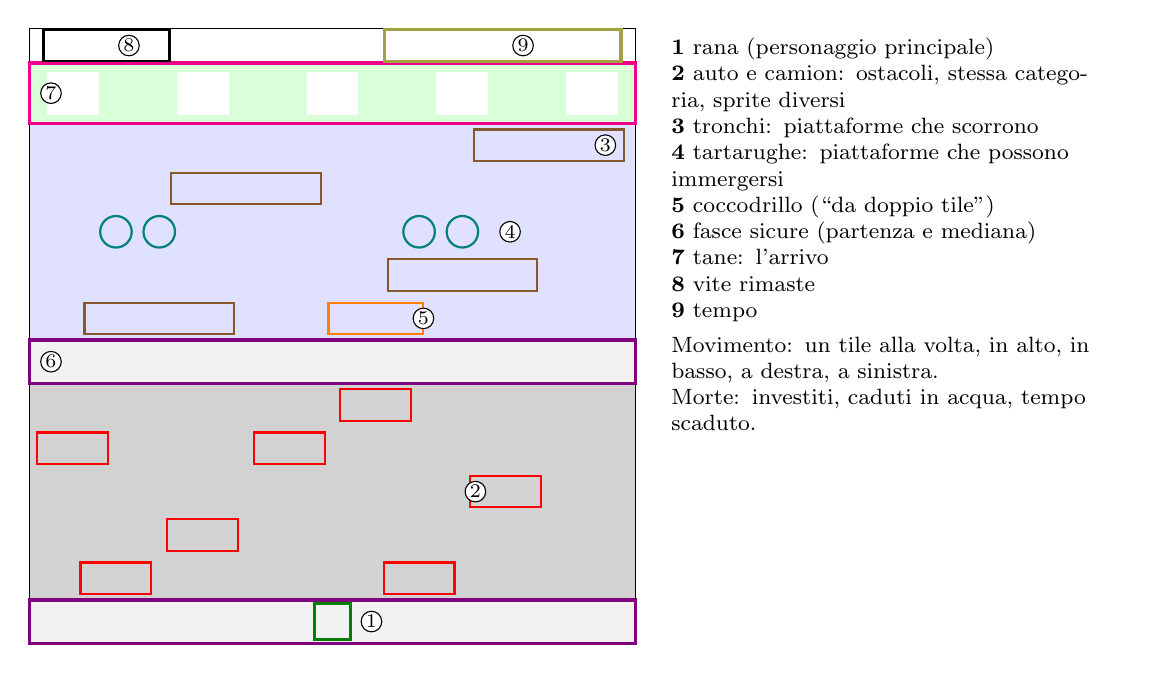
\begin{tikzpicture}[x=0.55cm, y=0.55cm, font=\scriptsize]
    % fasce dello schermo
    \fill[gray!10] (0,0) rectangle (14,1);       % partenza
    \fill[gray!35] (0,1) rectangle (14,6);       % strada
    \fill[gray!10] (0,6) rectangle (14,7);       % mediana
    \fill[blue!12] (0,7) rectangle (14,12);      % fiume
    \fill[green!15] (0,12) rectangle (14,13.4);  % tane
    \foreach \x in {1,4,7,10,13}
      \fill[white] (\x-0.6,12.2) rectangle (\x+0.6,13.2);
    \draw (0,0) rectangle (14,14.2);
    % elementi
    \node[draw=green!50!black, very thick, minimum size=0.45cm] (frog)
      at (7,0.5) {};
    \foreach \x/\y in {2/1.5, 9/1.5, 4/2.5, 11/3.5, 1/4.5, 6/4.5, 8/5.5}
      \node[draw=red, thick, minimum width=0.9cm, minimum height=0.4cm]
        at (\x,\y) {};
    \foreach \x/\y in {3/7.5, 10/8.5, 5/10.5, 12/11.5}
      \node[draw=brown!70!black, thick, minimum width=1.9cm,
        minimum height=0.4cm] at (\x,\y) {};
    \foreach \x/\y in {2/9.5, 3/9.5, 9/9.5, 10/9.5}
      \node[draw=teal, thick, circle, minimum size=0.4cm] at (\x,\y) {};
    \node[draw=orange, thick, minimum width=1.2cm, minimum height=0.4cm]
      at (8,7.5) {};
    \draw[violet, very thick] (0,6) rectangle (14,7);
    \draw[violet, very thick] (0,0) rectangle (14,1);
    \draw[magenta, very thick] (0,12) rectangle (14,13.4);
    \node[draw=black, thick, anchor=west, minimum width=1.6cm,
      minimum height=0.4cm] at (0.3,13.8) {};
    \node[draw=yellow!60!black, very thick, anchor=east,
      minimum width=3cm, minimum height=0.4cm] at (13.7,13.8) {};
    % numeri
    \foreach \n/\x/\y in {1/7.9/0.5, 2/10.3/3.5, 3/13.3/11.5, 4/11.1/9.5,
                          5/9.1/7.5, 6/0.5/6.5, 7/0.5/12.7, 8/2.3/13.8,
                          9/11.4/13.8}
      \node[circle, fill=white, draw, inner sep=0.5pt] at (\x,\y) {\n};
    % legenda
    \node[anchor=north west, align=left, text width=5.6cm,
      font=\footnotesize] at (14.6,14.2) {%
      \textbf{1} rana (personaggio principale)\\
      \textbf{2} auto e camion: ostacoli, stessa categoria, sprite
        diversi\\
      \textbf{3} tronchi: piattaforme che scorrono\\
      \textbf{4} tartarughe: piattaforme che possono immergersi\\
      \textbf{5} coccodrillo (``da doppio tile'')\\
      \textbf{6} fasce sicure (partenza e mediana)\\
      \textbf{7} tane: l'arrivo\\
      \textbf{8} vite rimaste\\
      \textbf{9} tempo\\[3pt]
      Movimento: un tile alla volta, in alto, in basso, a destra, a
      sinistra.\\
      Morte: investiti, caduti in acqua, tempo scaduto.};
  \end{tikzpicture}
  \caption{Ricostruzione schematica dell'esercizio del docente: lo schermo
  di \emph{Frogger} con gli elementi cerchiati in colori diversi e
  numerati, da affiancare alla lista delle regole. Non è lo screenshot
  originale; posizioni e numero degli oggetti sono indicativi.}
  \label{gd9:fig:frogger}
\end{figure}

\paragraph{Gli elementi cerchiati.} In ordine:
\begin{itemize}
  \item il \textbf{personaggio principale}, la rana;
  \item il \textbf{tempo}, che è una regola;
  \item gli \textbf{ostacoli} della strada: auto e camion, stessa categoria
        ma sprite diversi, ognuno cerchiato;
  \item i \textbf{coccodrilli}, ``sempre da doppio tile'', che andrebbero
        segnati con un altro colore. Lo screenshot scelto, però, non ne
        aveva uno ben visibile: ``avremmo dovuto scegliere uno screen con un
        coccodrillo, mia colpa'';
  \item le \textbf{tartarughe} e i \textbf{tronchi}, ciascuno con una
        meccanica specifica;
  \item le \textbf{tane}, cioè l'arrivo, e le caselle che servirebbero
        citate tutte;
  \item le \textbf{caselle viola}, che sono caselle neutre, sicure;
  \item le \textbf{vite} a schermo.
\end{itemize}
Sulle caselle il docente farebbe un discorso generale: la rana si muove
\textbf{di tile in tile}, sopra, sotto, a sinistra, a destra, ma sempre di un
tile alla volta; e ci sono tile \textbf{sicuri}. Uno studente ricorda le
\textbf{condizioni di morte}: ``assolutamente''. Il docente le segnerebbe in
maniera \textbf{visiva}.

\paragraph{L'immagine non è una decorazione.} Lo screenshot va messo accanto
al testo, ma non come decorazione: \textbf{interrompe il testo} perché
\textbf{è} il contenuto. Il docente prova a inserirlo in una tabella (``una
delle tabelle maledette''), che però si allarga troppo; alla fine lo mette in
coda alla sezione. Mangia metà pagina, ``e siamo d'accordo su questo''; ma
permette di \textbf{fare riferimento in modo specifico}, nelle regole, agli
elementi che si stanno già mostrando.

\paragraph{La legenda con i simboli colorati.} Manca un titolo, e la lista
andrebbe fatta come elenco puntato o tabella. Accanto a ogni voce, invece di
ripetere il nome, il docente inserisce un \textbf{carattere speciale} (un
quadratino) colorato come il contorno corrispondente nell'immagine, con una
nota del tipo \emph{element in the image}: una legenda più compatta e più
chiara. Con un'avvertenza: i \textbf{caratteri speciali}, quando il documento
viene esportato in PDF o stampato, potrebbero essere ``completamente
disintegrati'', e non apparire come li si vede sullo schermo. Per i task di
ora non è molto rilevante, ma va saputo.

\paragraph{Le interazioni e le risorse.} Lo stesso approccio vale per le
\textbf{interazioni}: si prende un'immagine del cabinato di \emph{Frogger}, si
ritagliano i controlli e si spiega a che cosa serve ciascuno (``e le
monetine a cosa servono?''). E per le \textbf{risorse}: le si cerchia tutte
con lo \textbf{stesso colore} e le si elenca nella sezione corrispondente.

\subsection{Una o due pagine}

``Si parte dalla lista; poi, quanto più riusciamo a renderla
\textbf{grafica}, visibile e comprensibile, meglio è.'' Questo è un modo, reso
possibile anche da un colpo di fortuna: Frogger è a schermata unica, quindi
quasi tutti gli elementi si possono citare su un'unica immagine. Andrebbe
spiegato meglio, ma come prima iterazione funziona: e si vede già come sia
\textbf{molto più chiaro}, e come in \textbf{una o due pagine} ``ce la
caviamo''. È lo stesso principio del \emph{mostrare invece di scrivere} visto
con i flowchart (sezione~\ref{sec:flowchart-usi}) e nelle revisioni del
primo task (sezione~\ref{rv:t1:sec:mostrare}).

% ---------------------------------------------------------------------
\section{La chiusura}
\label{gd9:sec:chiusura}

``Non abbiamo più tempo; anzi, vi ho tenuto qua anche troppo.'' Per le
domande, ci si scrive in privato o se ne parla. La lezione successiva è
\textbf{lunedì}, subito dopo il weekend, e si aprirà con le eventuali
domande. Se c'è qualcosa di ``imperativo, vitale'' da chiedere subito, il
docente resta qualche minuto; altrimenti, ``ci vediamo lunedì''.

% ---------------------------------------------------------------------
\section*{Punti chiave del capitolo}
\addcontentsline{toc}{section}{Punti chiave del capitolo}

\begin{itemize}
  \item Un task \textbf{non letto} è perso nel conteggio, ma si può
        \textbf{riconsegnare} (fino al 20\% dei task): copia o documento
        nuovo, mai modificare il vecchio né risolverne i commenti; integrare
        i propri commenti e quelli ai colleghi; cartella giusta, nome
        chiaro, avvisare il docente. Si riconsegna con ciò che si sa
        \emph{oggi}, e non il giorno dopo.
  \item Il limite dei \textbf{cinque errori grammaticali} può essere
        sollevato per chi ha dislessia o difficoltà simili, parlandone in
        privato; ma in un CV o in un portfolio quegli errori contano.
  \item La \textbf{libertà} non esiste come termine: si cerca
        l'\textbf{agency}, la capacità di esercitare potere \textbf{entro
        dei limiti} stabiliti dal designer (tre starter, quattro mosse, la
        build iniziale). Stun lock e crowd control la tolgono.
  \item Troppe scelte bloccano: \textbf{paura di scegliere} e
        \textbf{rimorso}; il cervello non regge i grandi numeri (fallacia di
        Monte Carlo). Il \emph{respec} aiuta, ma una scelta reversibile pesa
        meno.
  \item Il \textbf{paradosso della scelta} (Schwartz): più scelte, meno
        soddisfazione. Meno scelte ma \textbf{più profonde}: più soddisfazione,
        curva d'apprendimento più morbida, decisioni meaningful; meno costi,
        più iterazione, più creatività, più bilanciamento. Tre è un ottimo
        punto di partenza.
  \item La \textbf{Theory of Planned Behavior} spiega perché un
        comportamento viene adottato o no: \textbf{attitudine} (beneficial,
        enjoyable), \textbf{norme soggettive} (sociali, meta),
        \textbf{perceived behavioral control} (confidence, capability)
        portano all'\textbf{intenzione}; le \textbf{barriere} si frappongono
        tra intenzione e \textbf{comportamento}. Brilla nell'analisi da
        playtest.
  \item Formula semplificata: valori da $-10$ a $+10$; pesi di norma 1,
        fino a 2; $I = w_A(B+E) + w_N(S+M) + w_P\,\mathit{PBC}$; comportamento
        $= I + w_R R$ con $w_R$ pari al \textbf{doppio della media} dei
        pesi, perché le barriere si percepiscono più pesanti. Con pesi 1 e
        PBC accorpato: da $-70$ a $+70$.
  \item I valori vengono da designer e \textbf{utenza}: servono le
        demografiche, e bisogna chiedersi da dove vengono i dati (Reddit non
        è il mondo). Nei survey, \textbf{agency oculata}: risposte chiuse
        dove si può.
  \item Il \textbf{feedback} rinforza o riduce i comportamenti: datene il
        più possibile, per ciò che va bene e ciò che va male. È potente e,
        nei sistemi gacha, rischioso.
  \item Il \textbf{compendium} (design bible) è uno per progetto: una mappa
        di link a tutti i documenti, divisa per dipartimento, con
        \textbf{status} (e legenda), essenziale, accessibile a tutti,
        aggiornata dai lead.
  \item I \textbf{pilastri} sono \textbf{tre}, ad alto livello,
        inequivocabili (God of War: \emph{Combat}, \emph{Father/Son},
        \emph{Exploration}); il team li deve avere sempre sotto gli occhi.
  \item La \textbf{vision} formalizza i pilastri: prime emotions e moods (tre
        ciascuno), eventualmente obiettivo e morale, \textbf{must do},
        \textbf{must not}, \textbf{nice to have}, al massimo tre
        \textbf{USP}. Una volta approvata dalla direzione è
        \textbf{blindata}; funzione prima della forma.
  \item La \textbf{team vision} fissa missione, tipo di produzione, PR,
        gerarchia, pipeline, diritti e doveri: si firma, e si scrive
        \textbf{onestamente}.
  \item Le risposte di fine pre-produzione stanno nella \textbf{somma} dei
        documenti. I documenti mostrati sono \textbf{linee guida}, non
        template: ora è il momento di sperimentare.
  \item Nei core elements di \emph{Frogger}: game qualities come sistemi di
        alto livello; il timing è una dinamica, non un obiettivo; niente
        celle vuote (TBD o barra); titoli con stili veri; tabelle con
        giudizio; il tema in un box; uno screenshot annotato al posto di un
        muro di regole.
\end{itemize}
